\chapter{Implementation}

This chapter presents the implementation of the AI-Powered Online Exam Proctoring System, including the development tools, user interfaces, and core functionalities for different user roles.

\section{Overview}

The system is implemented as a full-stack web application using React 19.0 for the frontend and Flask 3.1.1 for the backend. It integrates YOLOv8n for object detection and MediaPipe for facial analysis to enable automated proctoring during online examinations. The system supports real-time video streaming using WebRTC technology with dual camera support (desktop and mobile). The implementation provides three distinct user interfaces: Admin Interface (system management, user administration, analytics), Teacher Interface (exam creation, student monitoring, result management), and Student Interface (exam participation with real-time proctoring).

\section{The Development Tool}

The development utilized modern tools and technologies: \textbf{Frontend} - React 19.0 with Tailwind CSS, Vite build tool, Socket.IO Client, React Router v6; \textbf{Backend} - Python 3.12 with Flask 3.1.1, Flask-SocketIO, PyJWT 2.10.1, Bcrypt 4.3.0, Gunicorn; \textbf{AI/ML} - PyTorch 2.7.1, Ultralytics YOLOv8n, MediaPipe 0.10.21, OpenCV 4.11; \textbf{Database} - MySQL 8.0, Visual Studio Code, Git/GitHub, Swagger/Flasgger, Sentry SDK.

\section{Welcome Page and User Login}

The welcome page serves as the landing interface featuring a clean, modern design with gradient background, system branding, key feature highlights (real-time AI proctoring, dual camera support, instant alerts), and call-to-action buttons. The login system provides secure JWT-based authentication with role-based access control where users select their role (Admin/Teacher/Student) and enter credentials. Security features include bcrypt password hashing, rate limiting, input sanitization, and CSRF protection.

\begin{figure}[p]
    \centering
    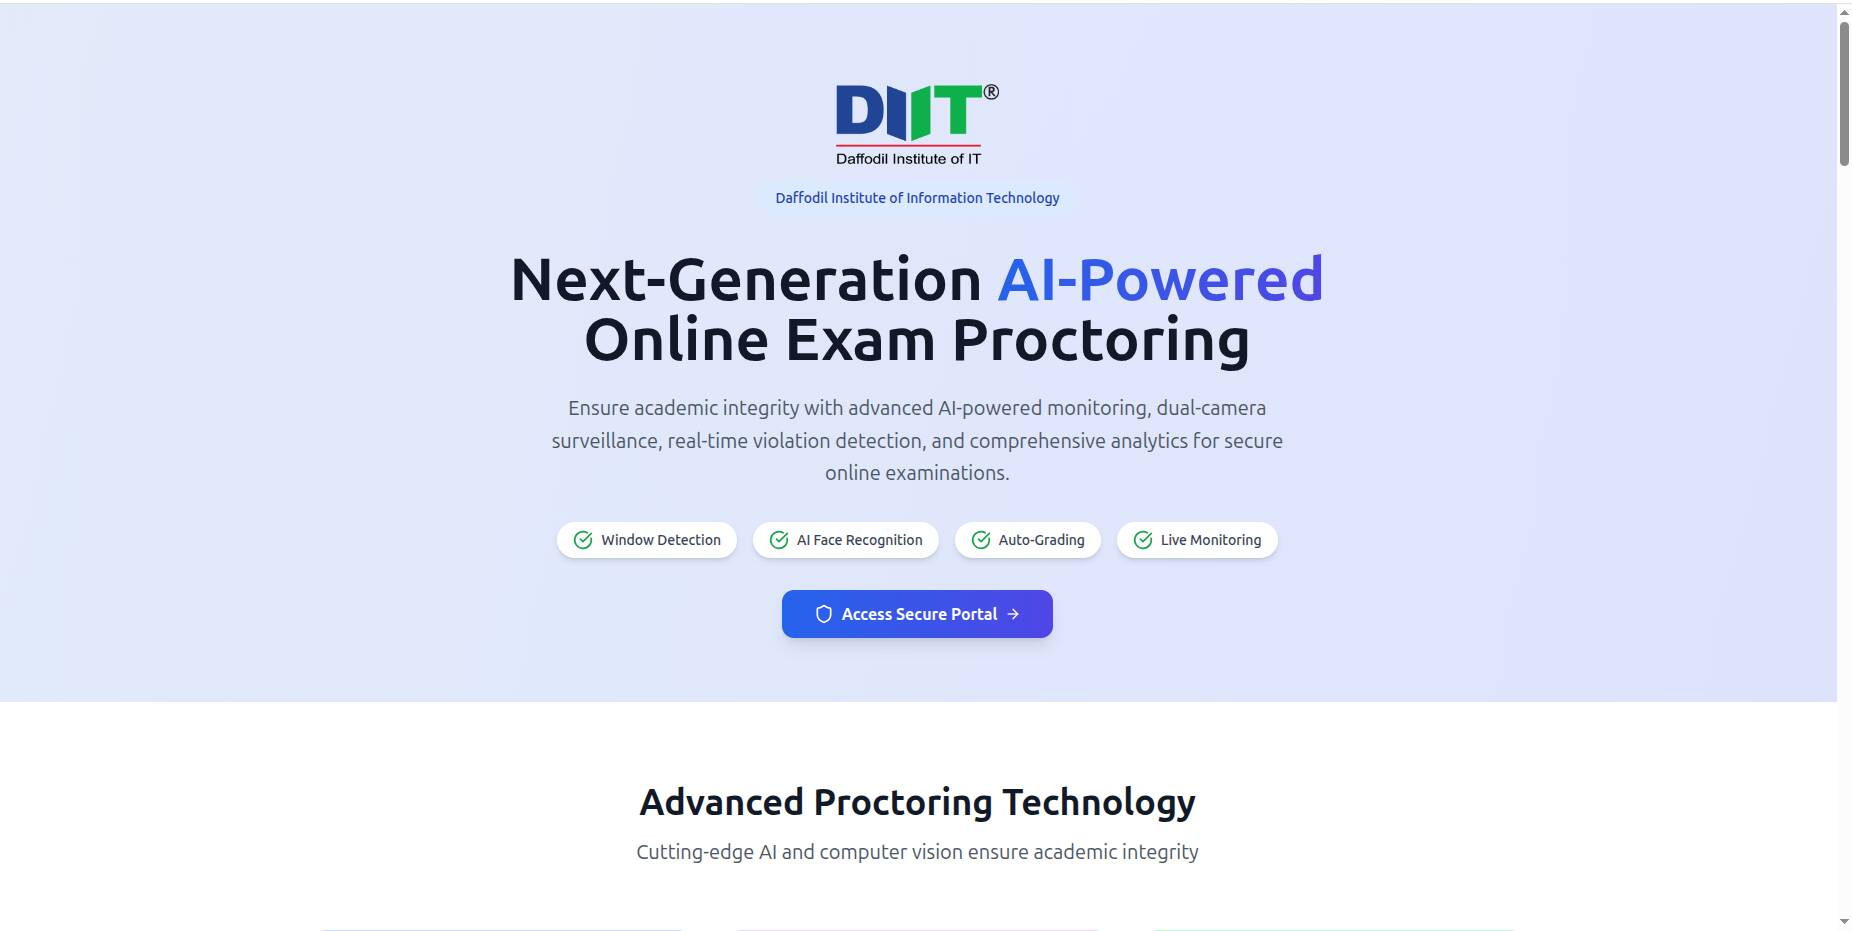
\includegraphics[width=0.7\textwidth]{Chap4/welcome_page.jpg}
    \caption{Welcome Page - Landing Interface}
    \label{fig:welcome_page}
\end{figure}

\begin{figure}[p]
    \centering
    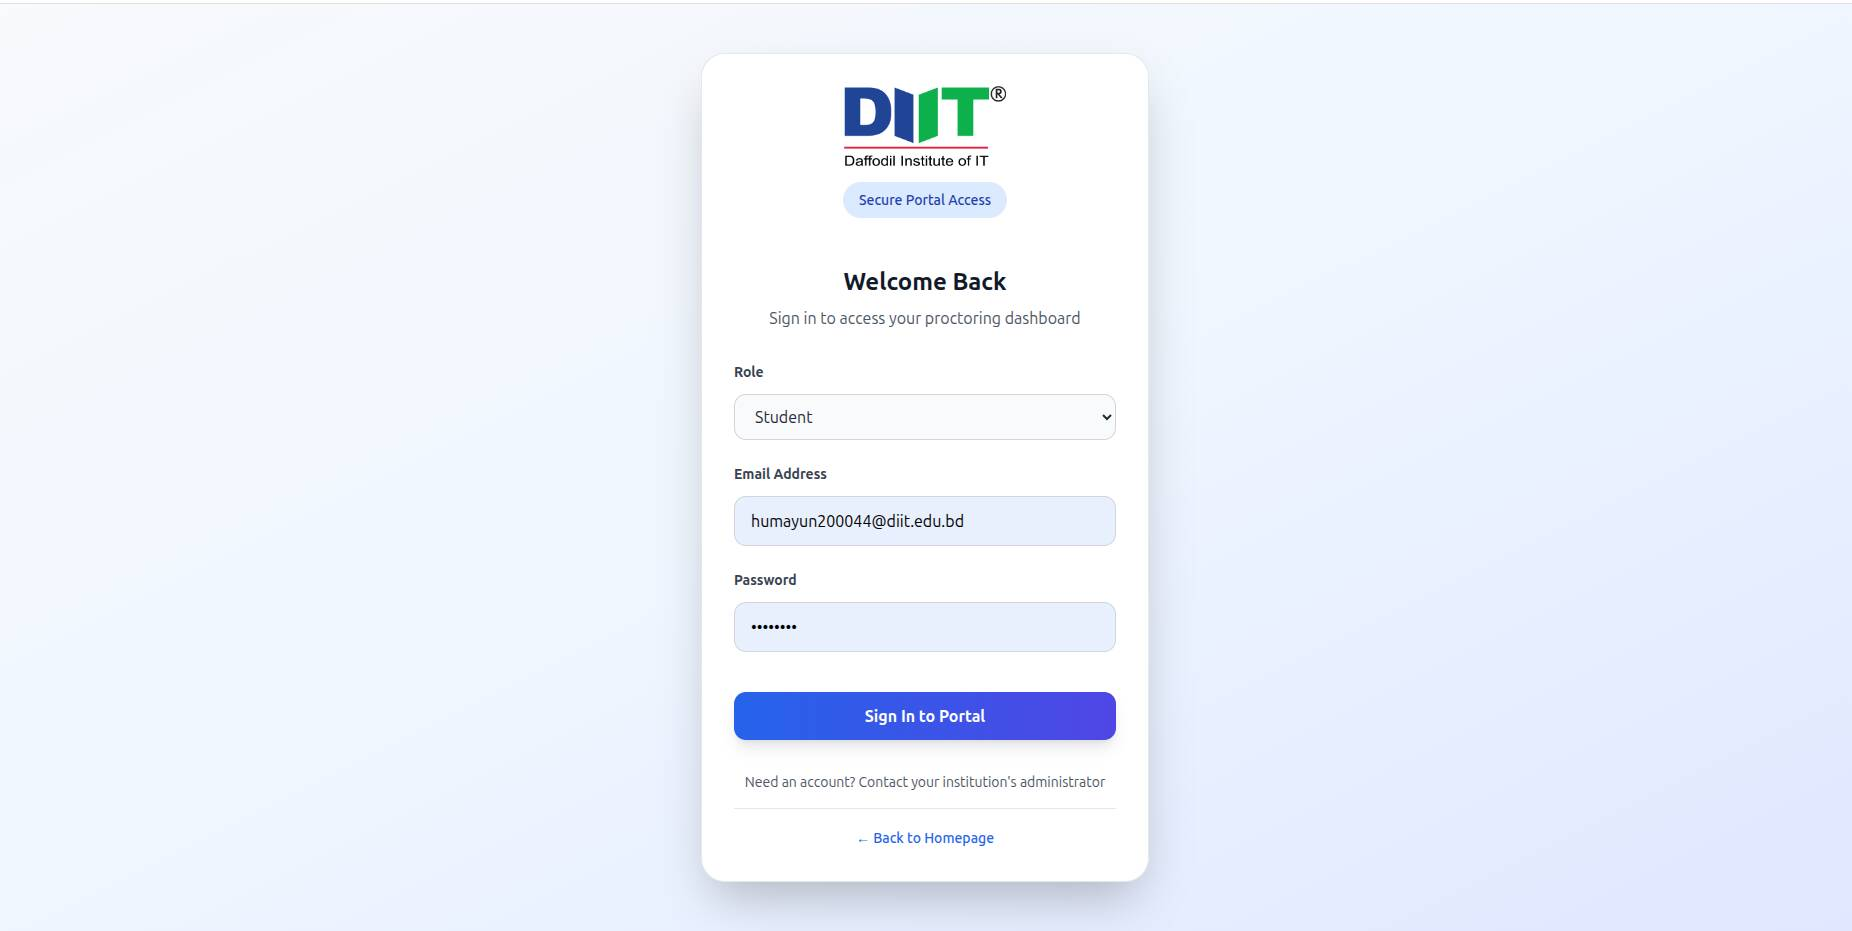
\includegraphics[width=0.7\textwidth]{Chap4/login_page.jpg}
    \caption{User Login Page}
    \label{fig:login_page}
\end{figure}

\section{Admin Dashboard}

The Admin Dashboard provides comprehensive system management with full control over users, exams, and configuration. The dashboard displays key statistics including total students, teachers, exams, active exams, and violations detected with sidebar navigation, main content area, and header bar.

\begin{figure}[p]
    \centering
    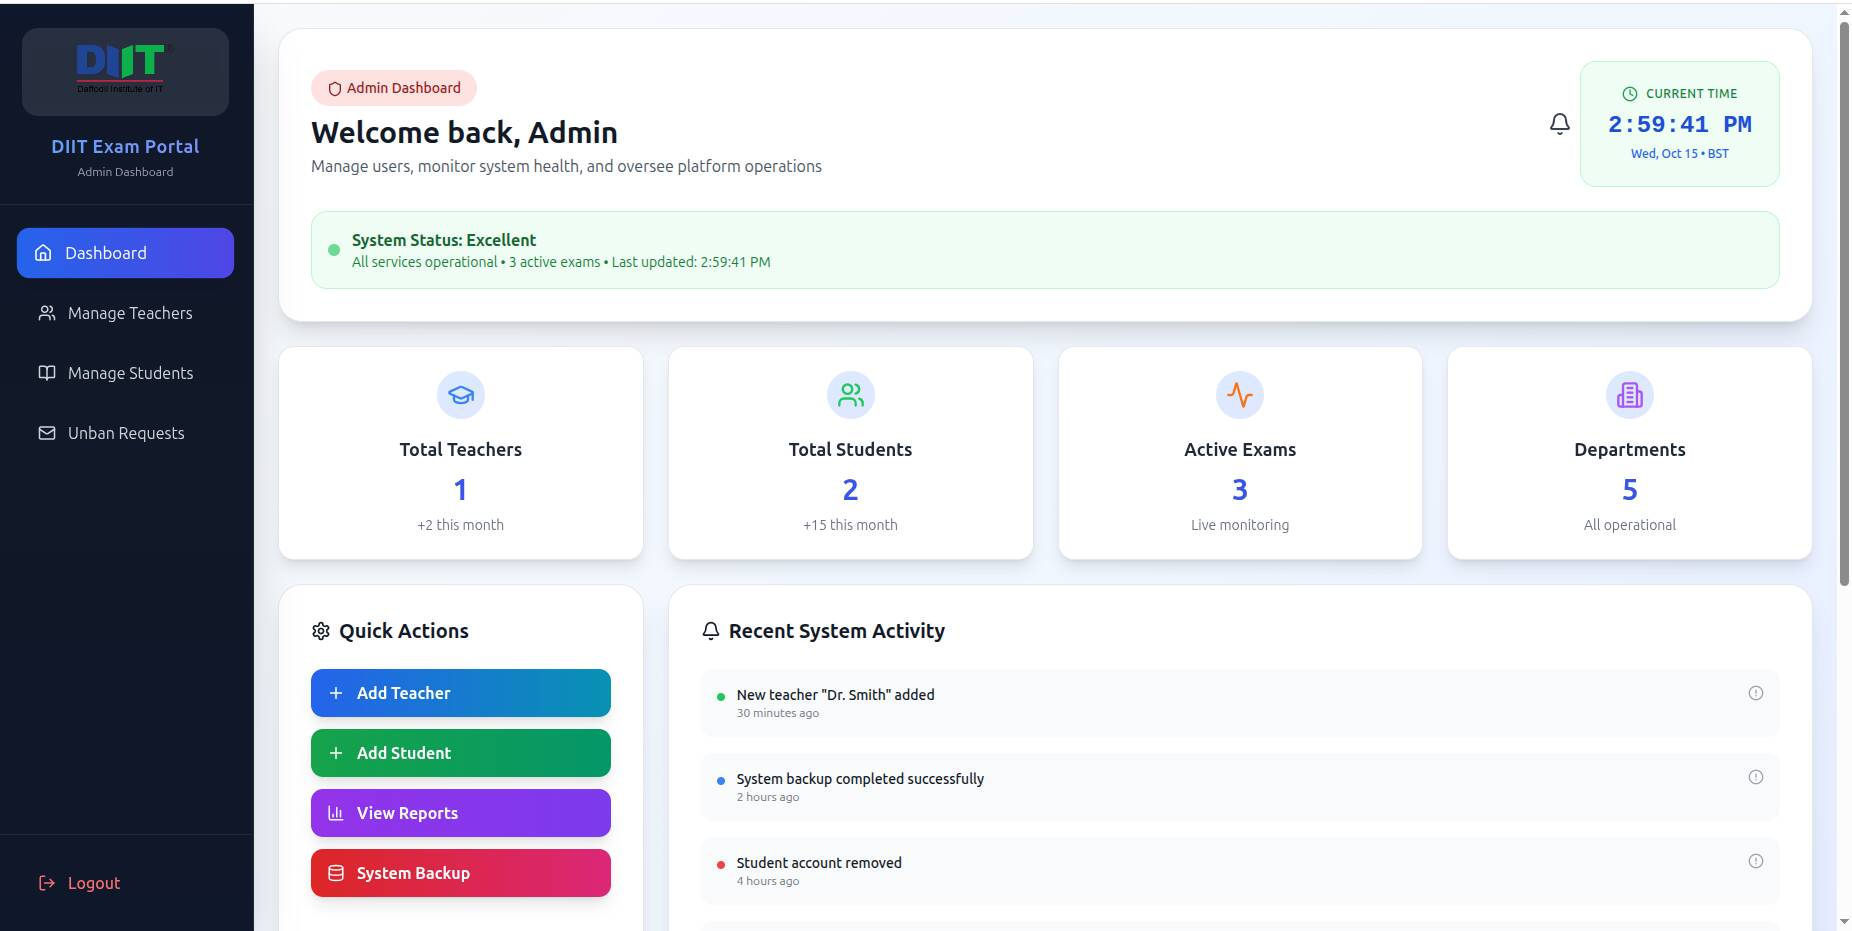
\includegraphics[width=0.8\textwidth]{Chap4/admin_dashboard_overview.jpg}
    \caption{Admin Dashboard Overview}
    \label{fig:admin_dashboard}
\end{figure}

\subsection{Student Management}

Administrators manage student accounts with CRUD operations, paginated tables with search/filters, bulk operations (CSV import/export), and detailed profile views. The add student form captures personal information, academic details (roll number, department, batch, section, semester), and account settings.

\begin{figure}[p]
    \centering
    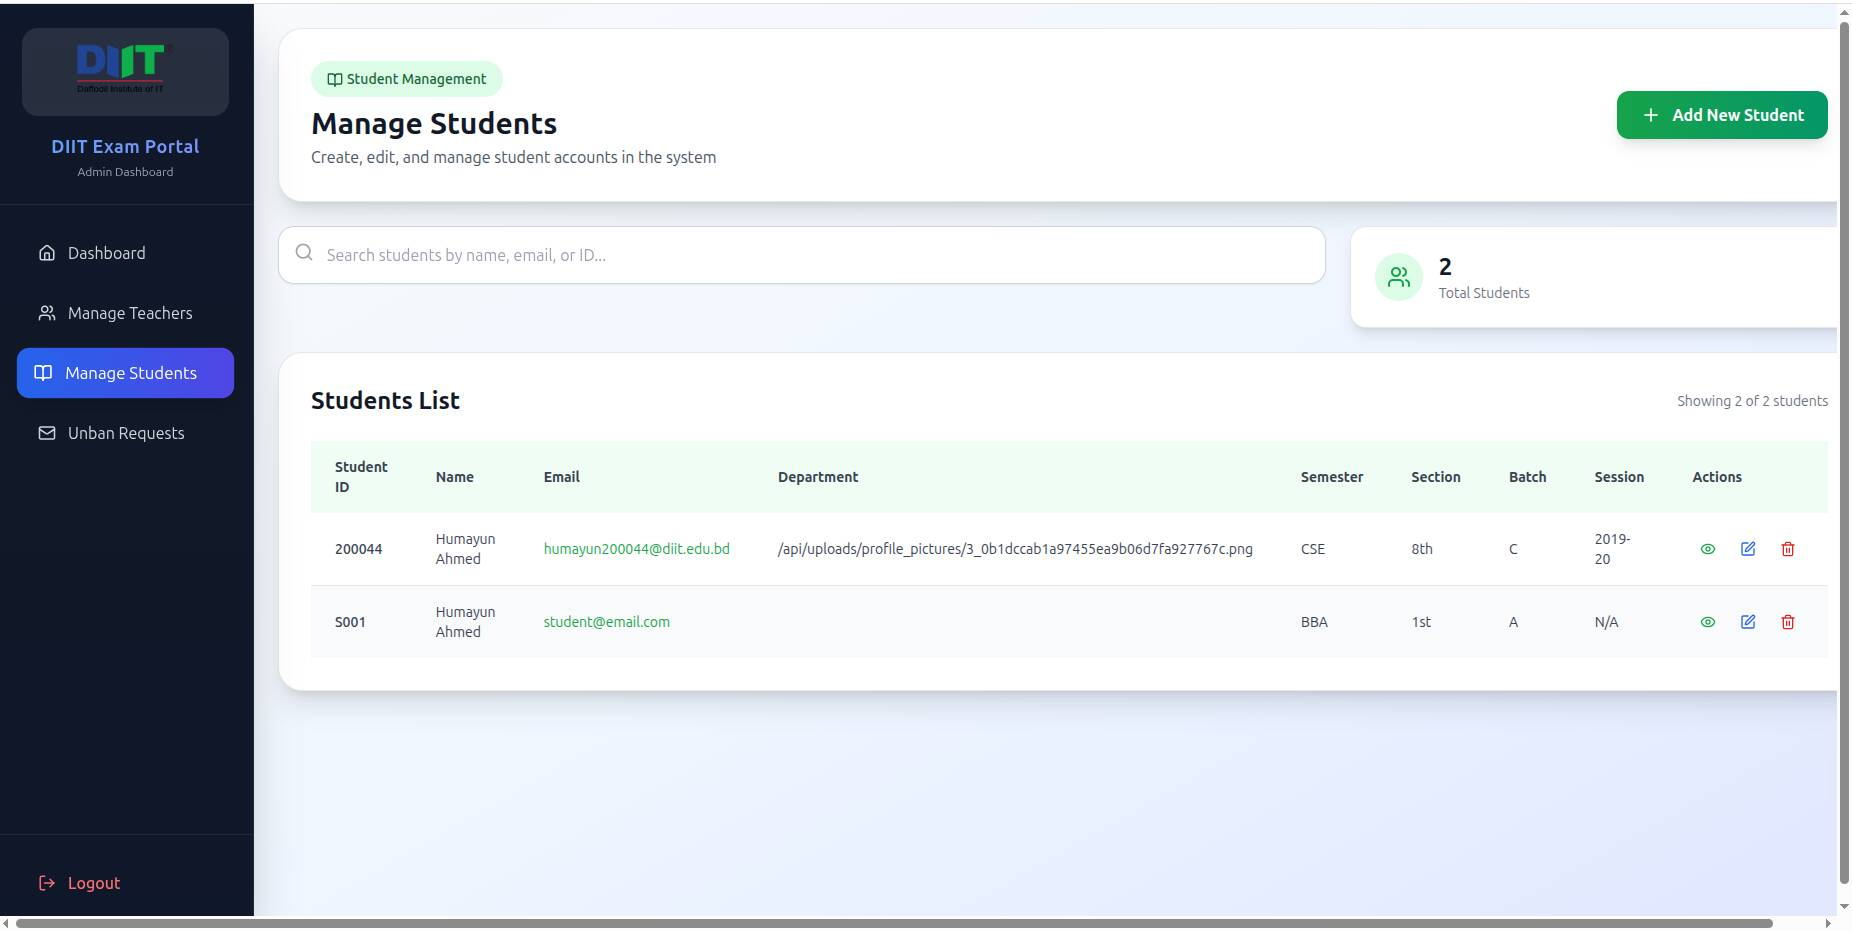
\includegraphics[width=0.7\textwidth]{Chap4/admin_student_management.jpg}
    \caption{Student Management Interface}
    \label{fig:admin_students}
\end{figure}

\begin{figure}[p]
    \centering
    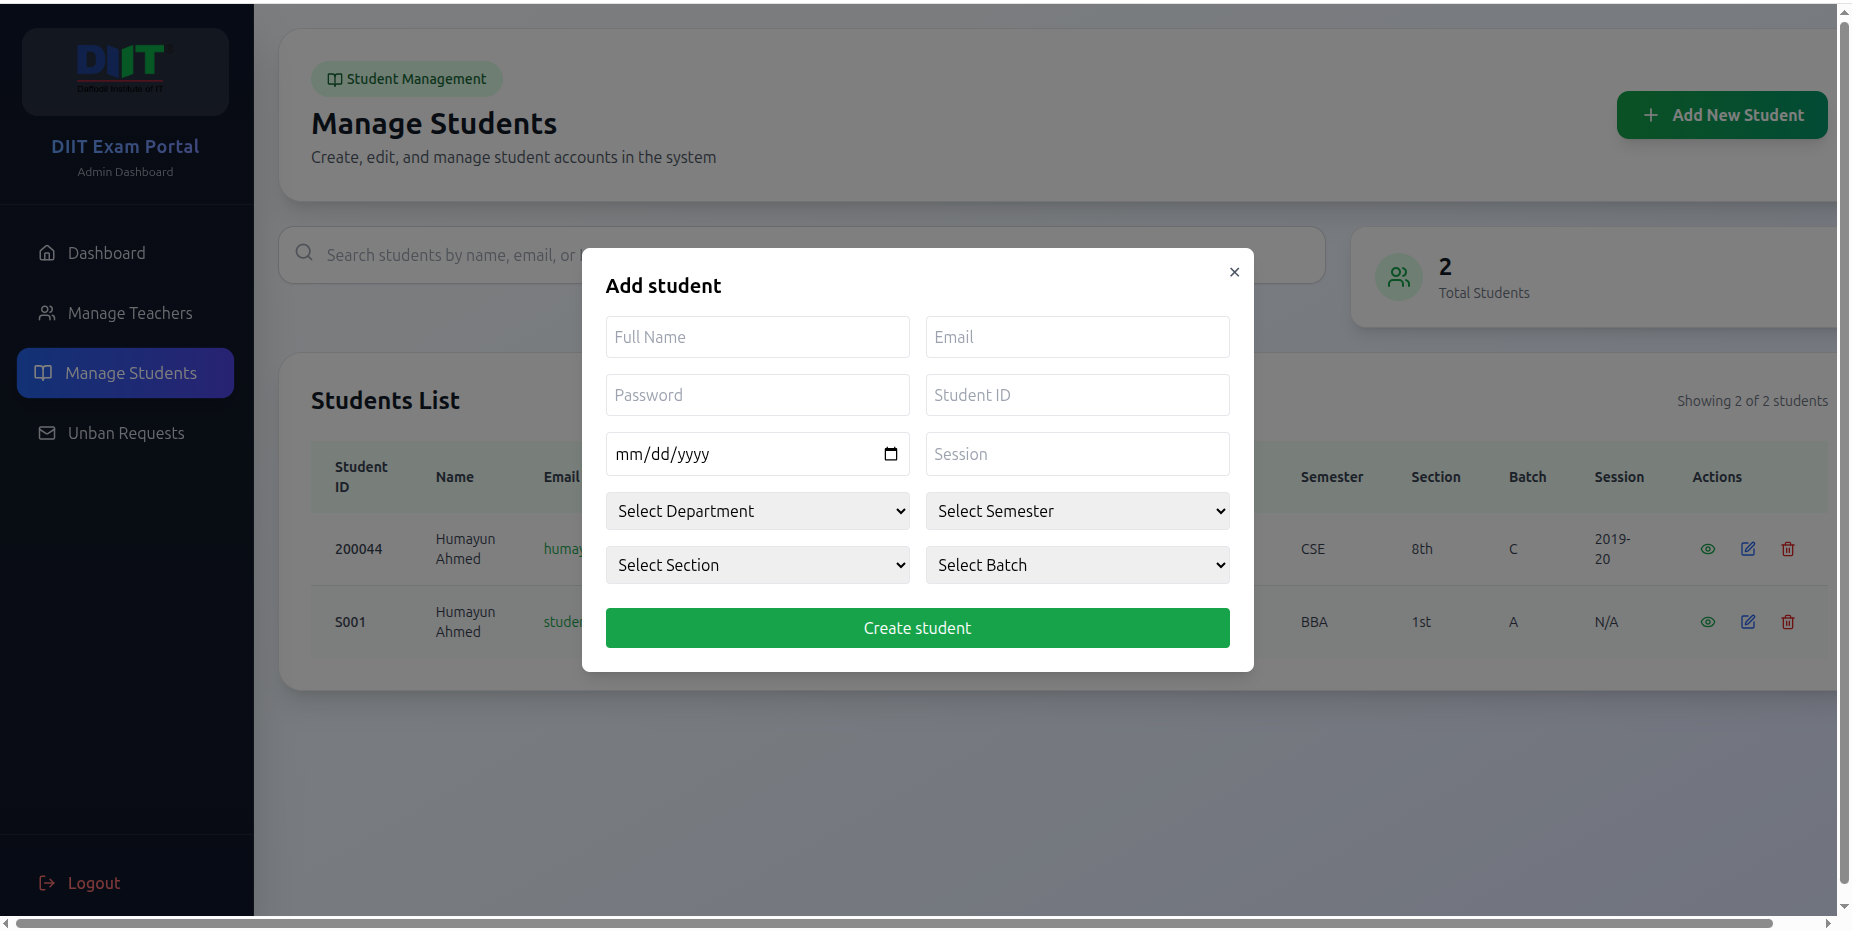
\includegraphics[width=0.7\textwidth]{Chap4/admin_add_student.png}
    \caption{Add Student Form}
    \label{fig:admin_add_student}
\end{figure}

\subsection{Teacher Management}

Similar capabilities for managing teacher accounts including viewing teachers with course assignments, adding new teachers, editing profiles, and assigning courses.

\begin{figure}[p]
    \centering
    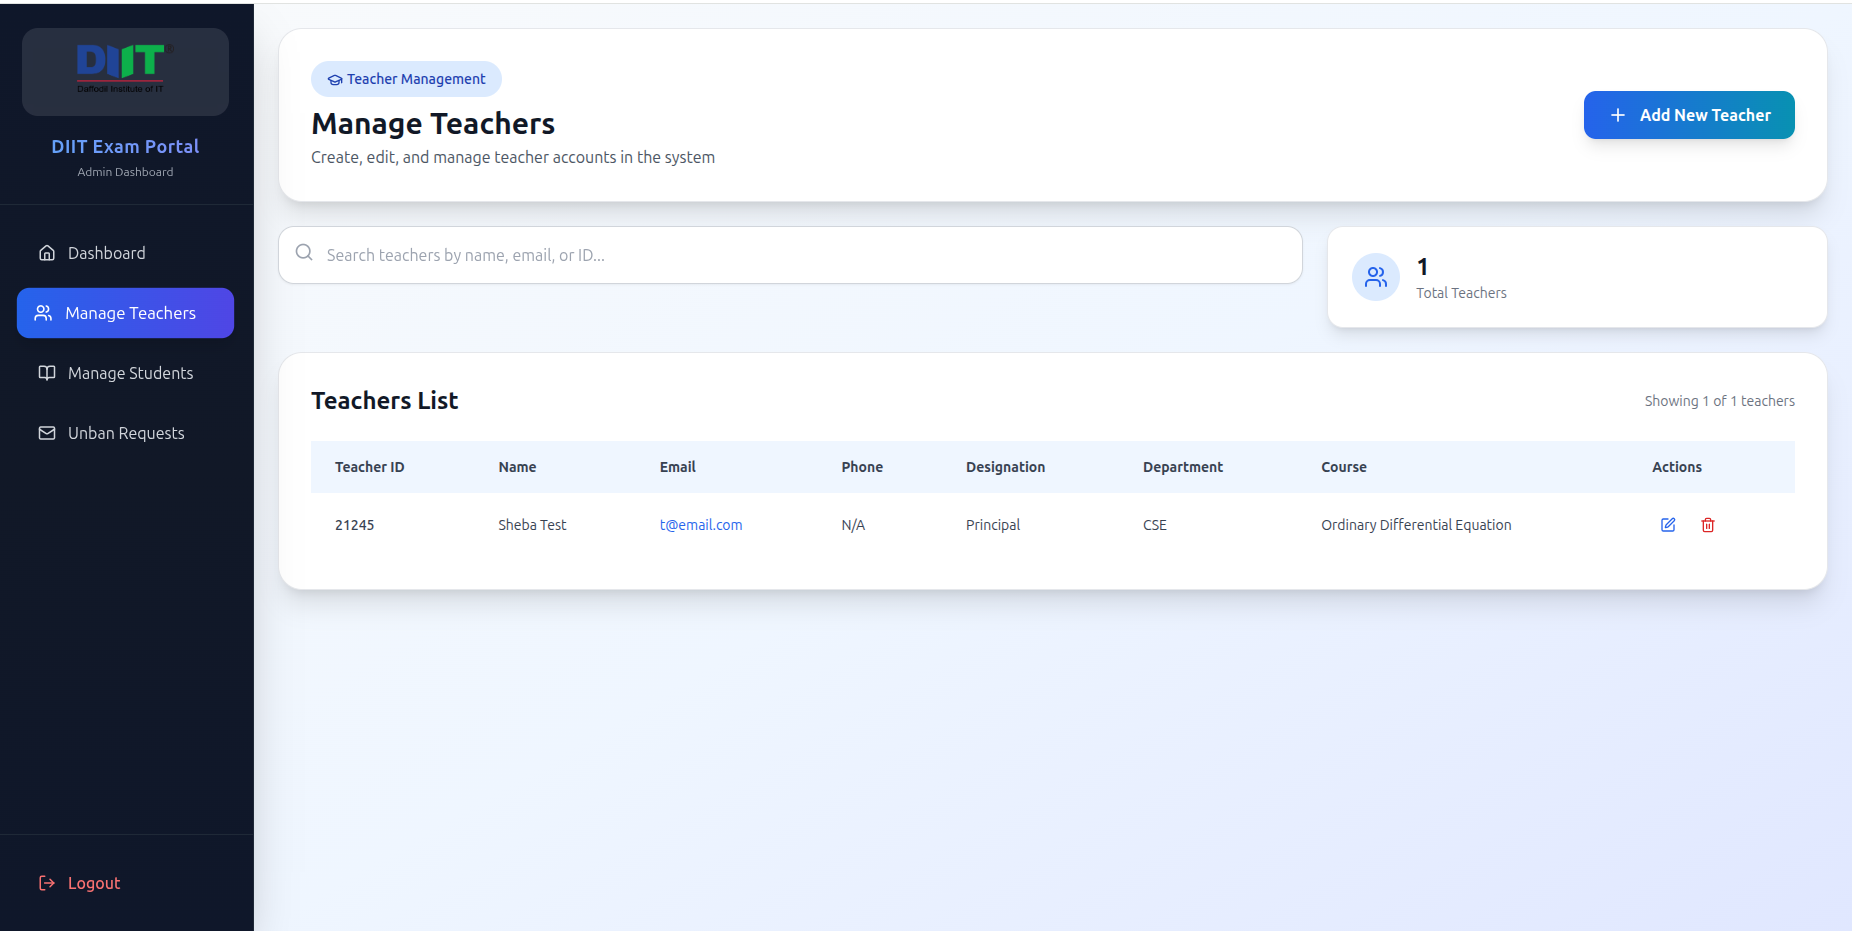
\includegraphics[width=0.7\textwidth]{Chap4/admin_teacher_management.png}
    \caption{Teacher Management Interface}
    \label{fig:admin_teachers}
\end{figure}

\begin{figure}[p]
    \centering
    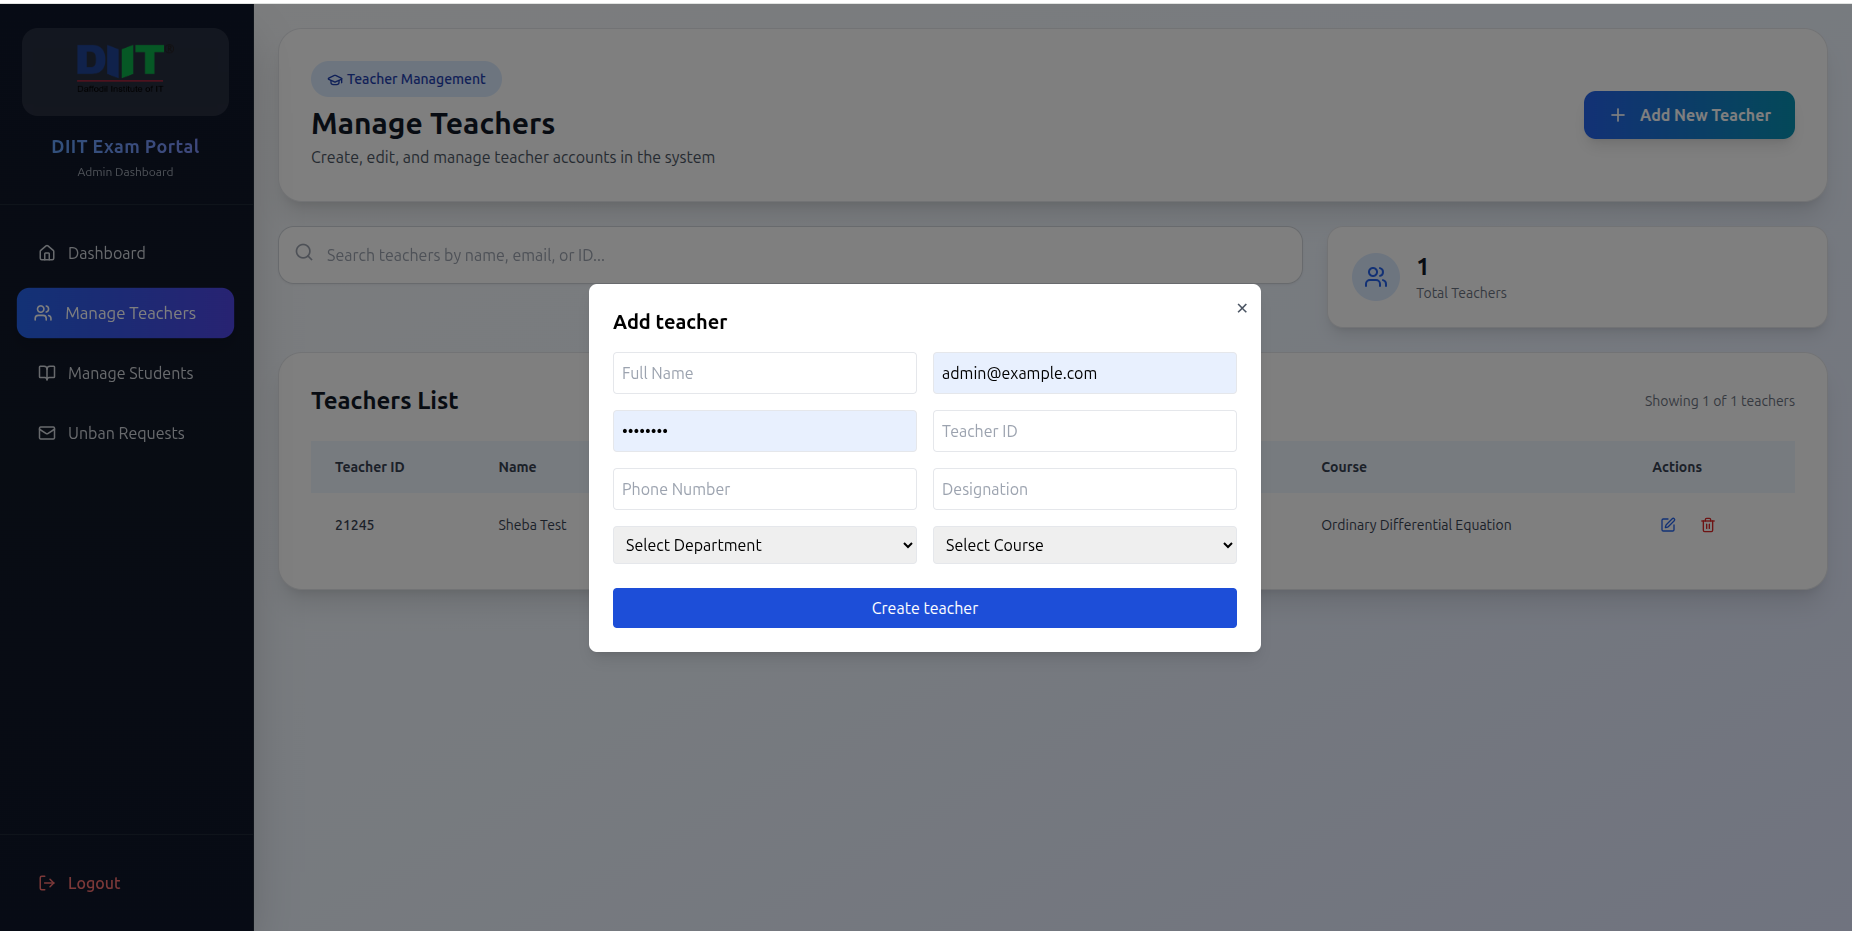
\includegraphics[width=0.7\textwidth]{Chap4/admin_add_teacher.png}
    \caption{Add Teacher Form}
    \label{fig:admin_add_teacher}
\end{figure}

\section{Teacher Dashboard}

The Teacher Dashboard enables faculty to create exams, monitor students in real-time, and manage results. Teachers see quick statistics, recent activity, quick action buttons, and a calendar view of scheduled exams.

\begin{figure}[p]
    \centering
    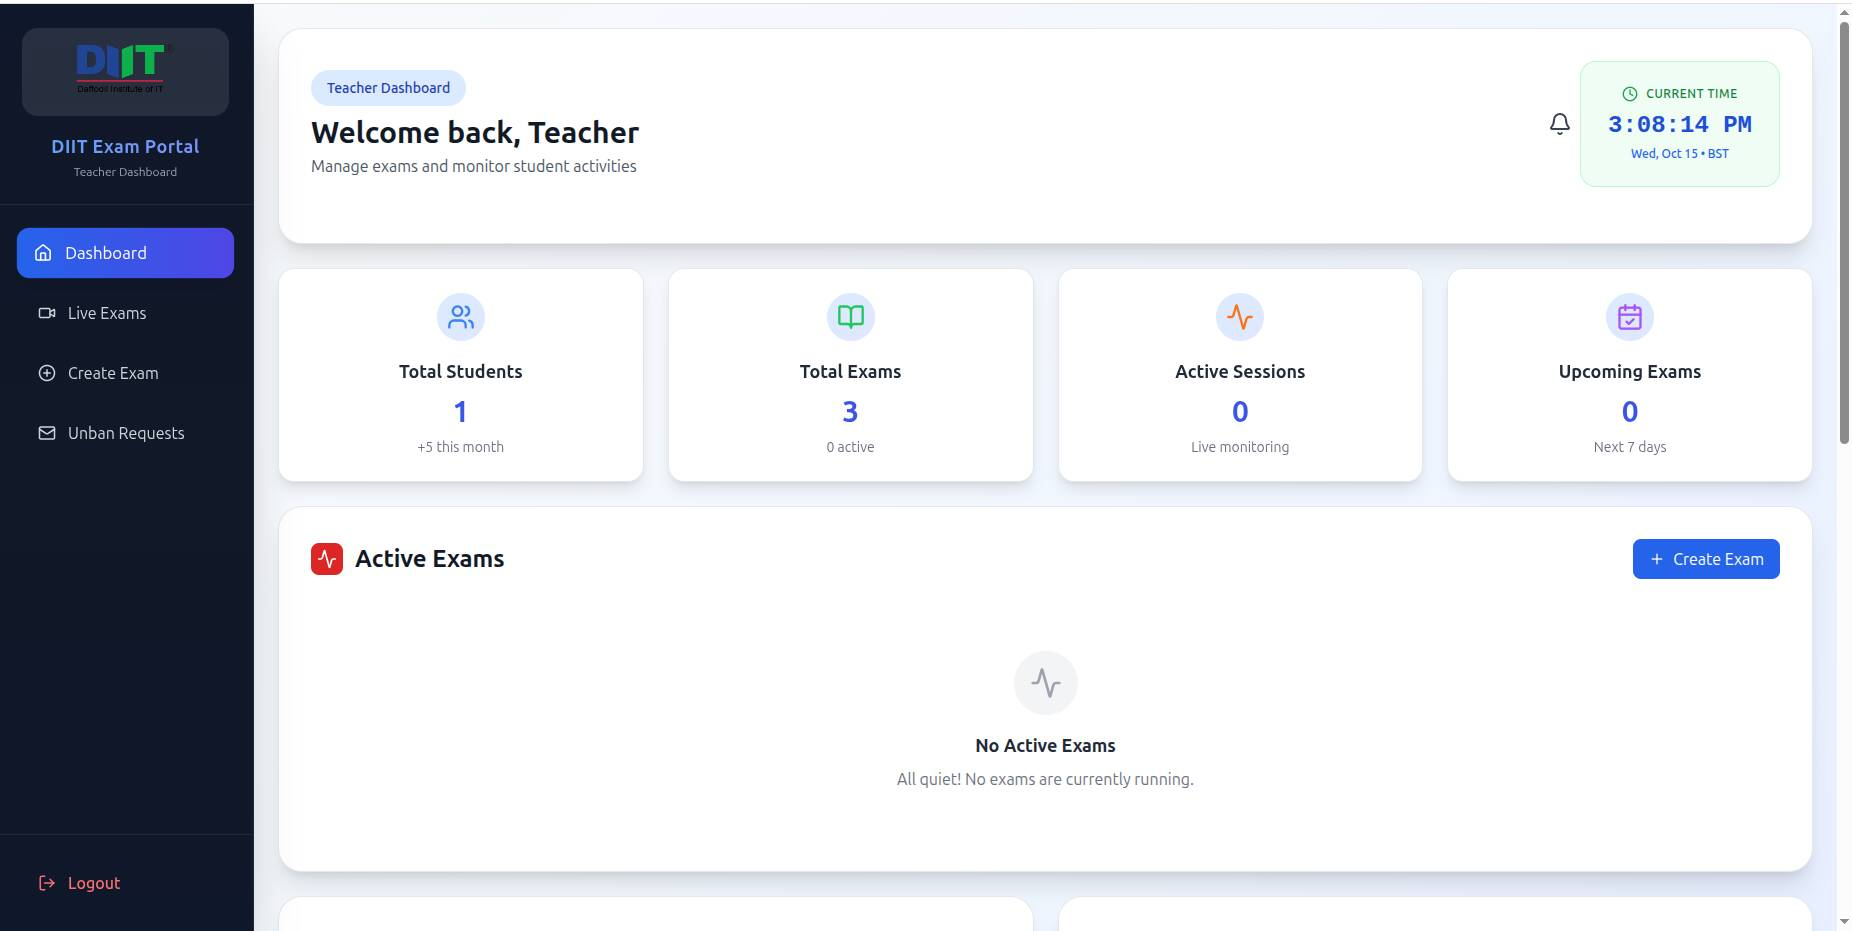
\includegraphics[width=0.8\textwidth]{Chap4/teacher_dashboard_overview.jpg}
    \caption{Teacher Dashboard Overview}
    \label{fig:teacher_dashboard}
\end{figure}

\subsection{Create Exam and Manage Exams}

The exam creation uses a multi-step form for basic information, question configuration, and proctoring settings. The multi-step process includes: (1) Basic Information - exam title, course selection, date/time scheduling, academic filters (department, batch, section, semester); (2) Question Configuration - adding MCQ and written questions with marks allocation; (3) Proctoring Settings - configuring detection sensitivity, violation thresholds, camera requirements; (4) Review and Publish. Teachers manage exams in a tabbed interface showing Upcoming, Live, Completed, and Draft exams with options to edit, clone, delete, view results, and download reports.

\begin{figure}[p]
    \centering
    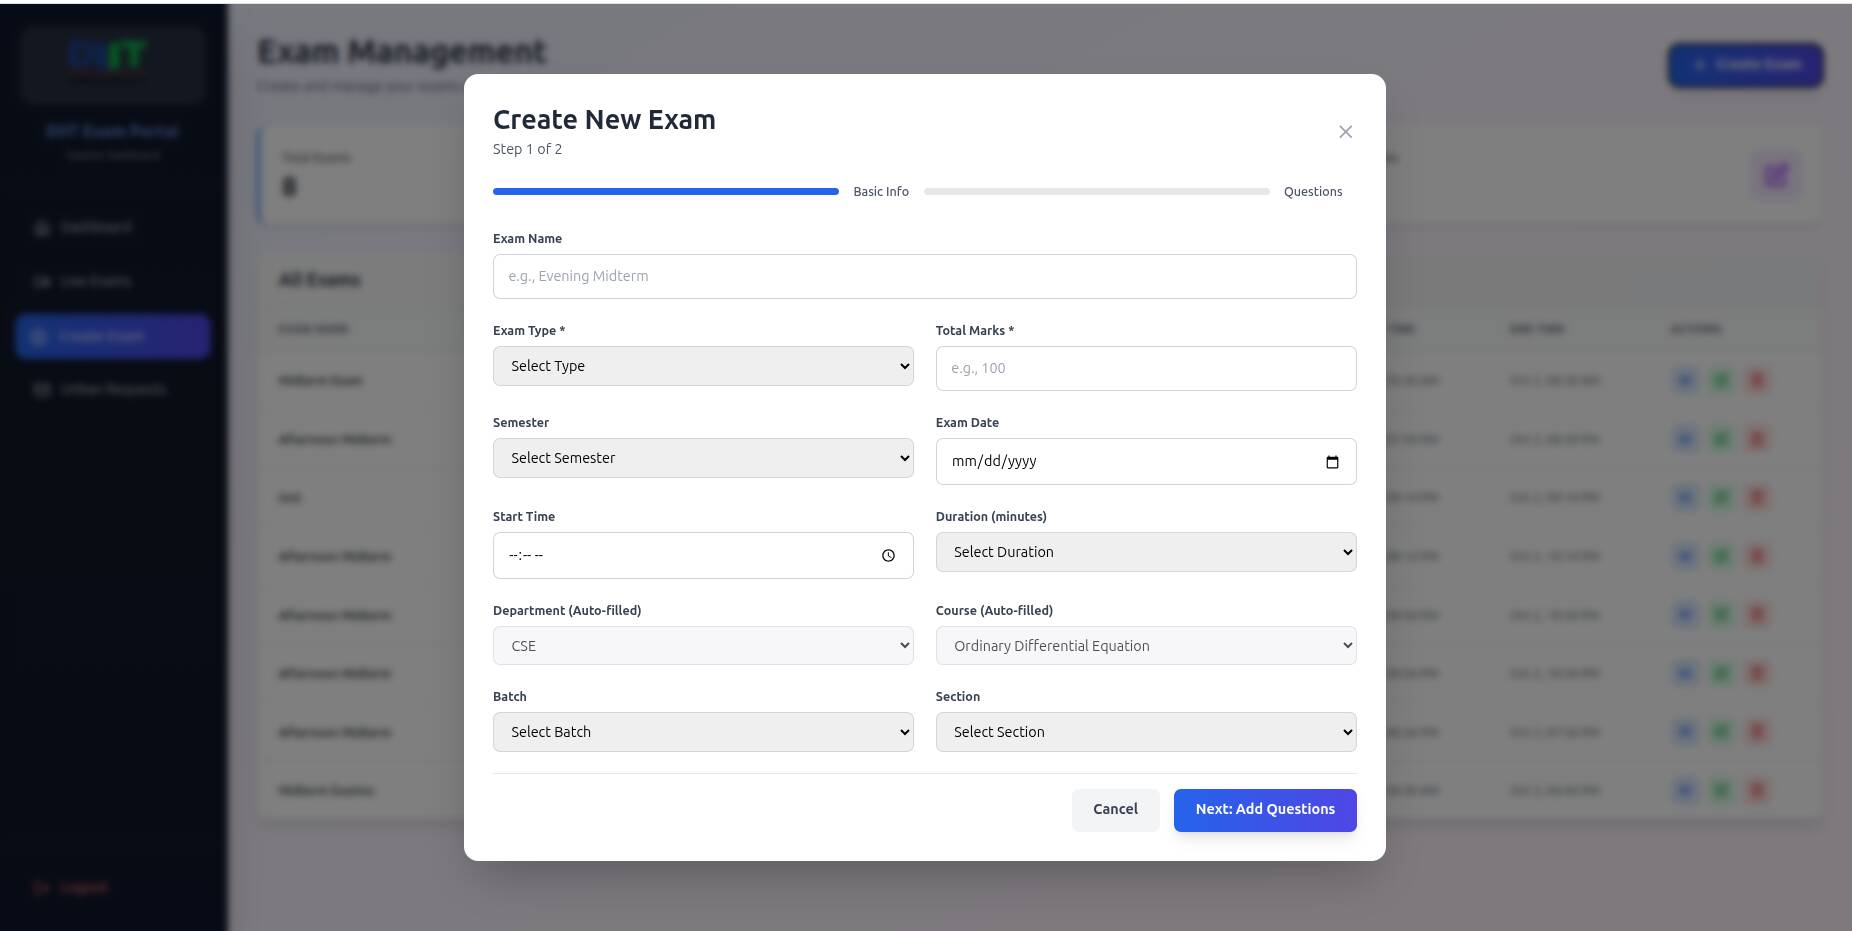
\includegraphics[width=0.7\textwidth]{Chap4/teacher_create_exam.jpg}
    \caption{Create Exam Interface - Multi-step Form}
    \label{fig:teacher_create}
\end{figure}

\begin{figure}[p]
    \centering
    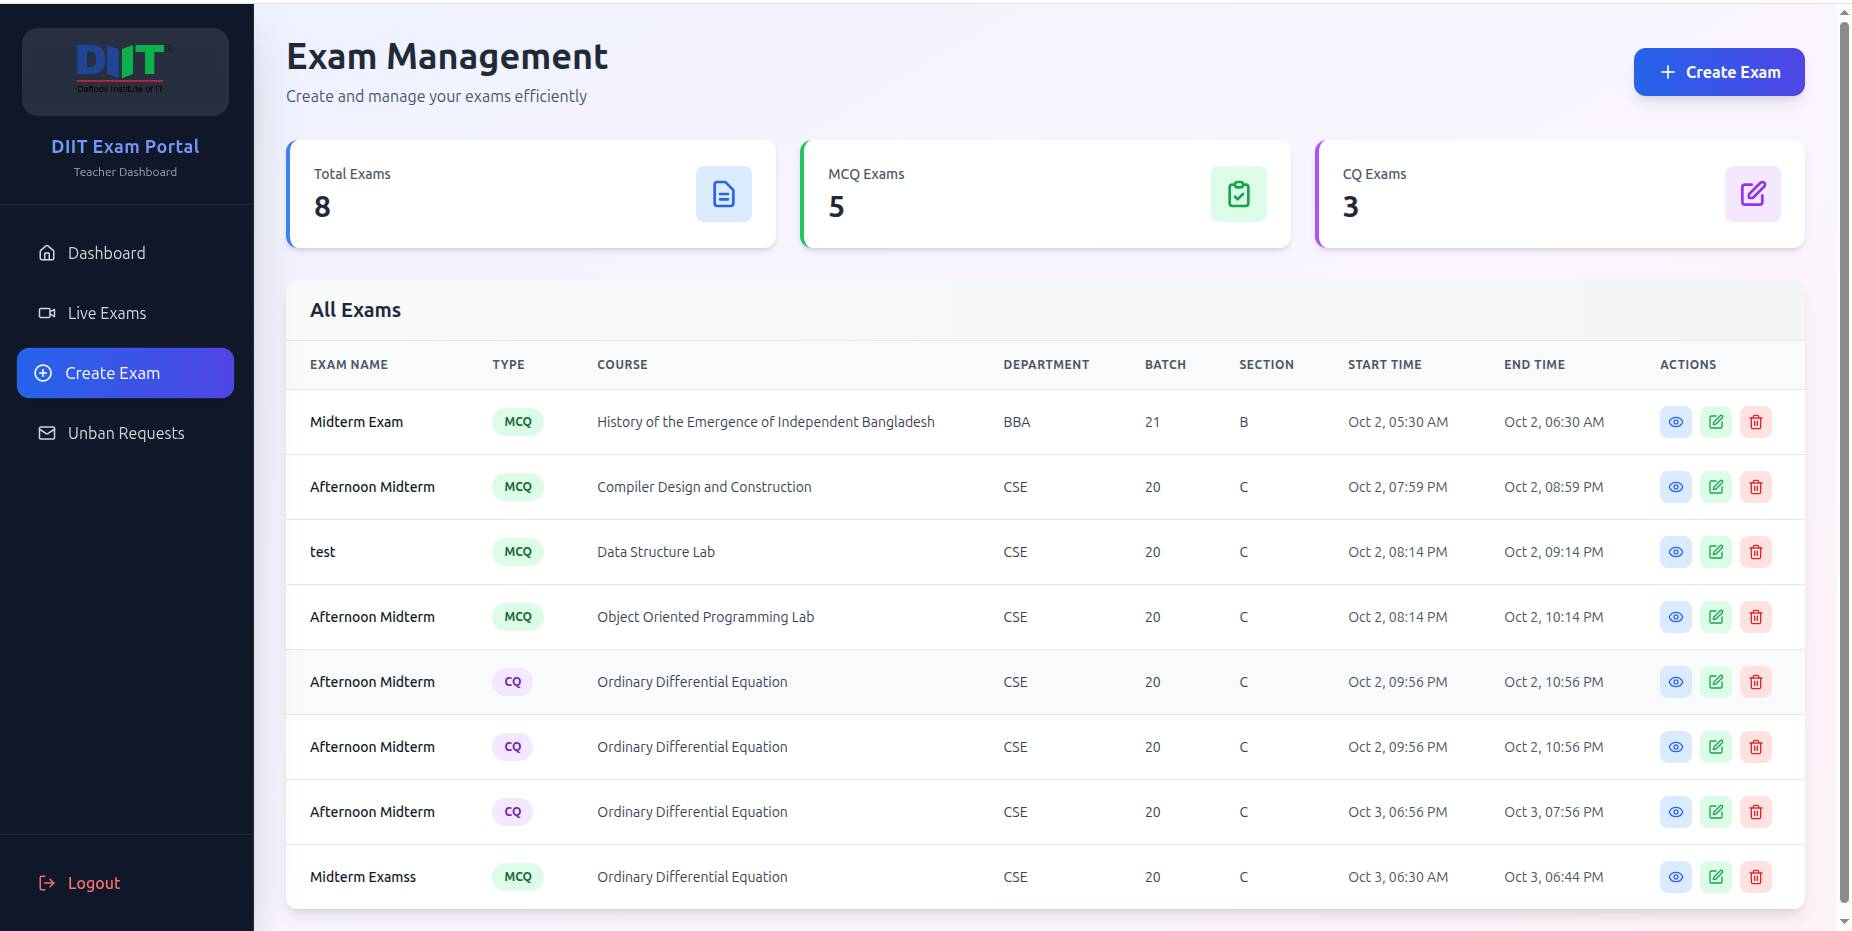
\includegraphics[width=0.7\textwidth]{Chap4/teacher_my_exams.jpg}
    \caption{My Exams List - Management Interface}
    \label{fig:teacher_exams}
\end{figure}

\subsection{Live Monitoring}

Real-time monitoring displays student grid view with video thumbnails and violation tracking. The monitoring interface shows live video feeds from all students taking the exam, with color-coded status indicators (green for normal, yellow for warnings, red for violations), violation count badges, and aggregate statistics showing total students, active students, and total violations detected.

\begin{figure}[p]
    \centering
    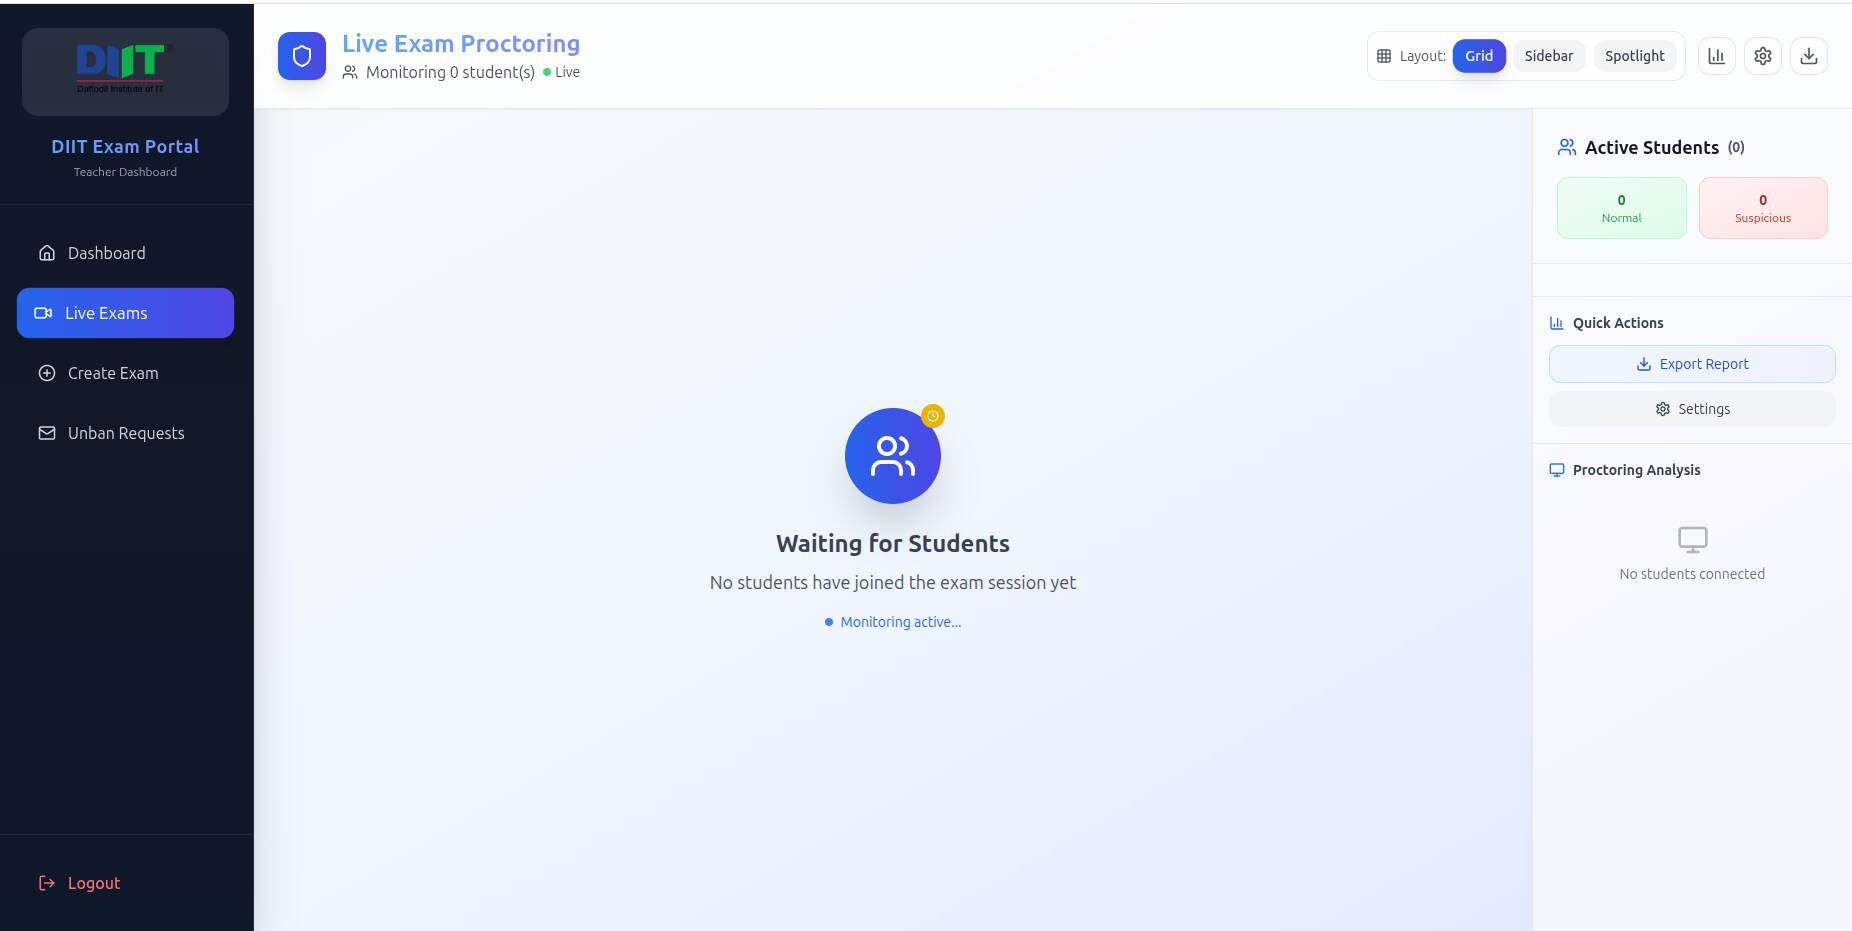
\includegraphics[width=0.8\textwidth]{Chap4/teacher_live_monitoring_grid.jpg}
    \caption{Live Monitoring Grid - Real-time Student Surveillance}
    \label{fig:teacher_monitor}
\end{figure}

\subsection{Results and Student Management}

Teachers access results interface with summary statistics and export functionality. The results interface displays exam performance metrics, individual student scores, automated grading for MCQs, and manual grading interface for written responses with feedback options. The student management section shows all students in assigned sections with detailed profiles and performance analytics.

\begin{figure}[p]
    \centering
    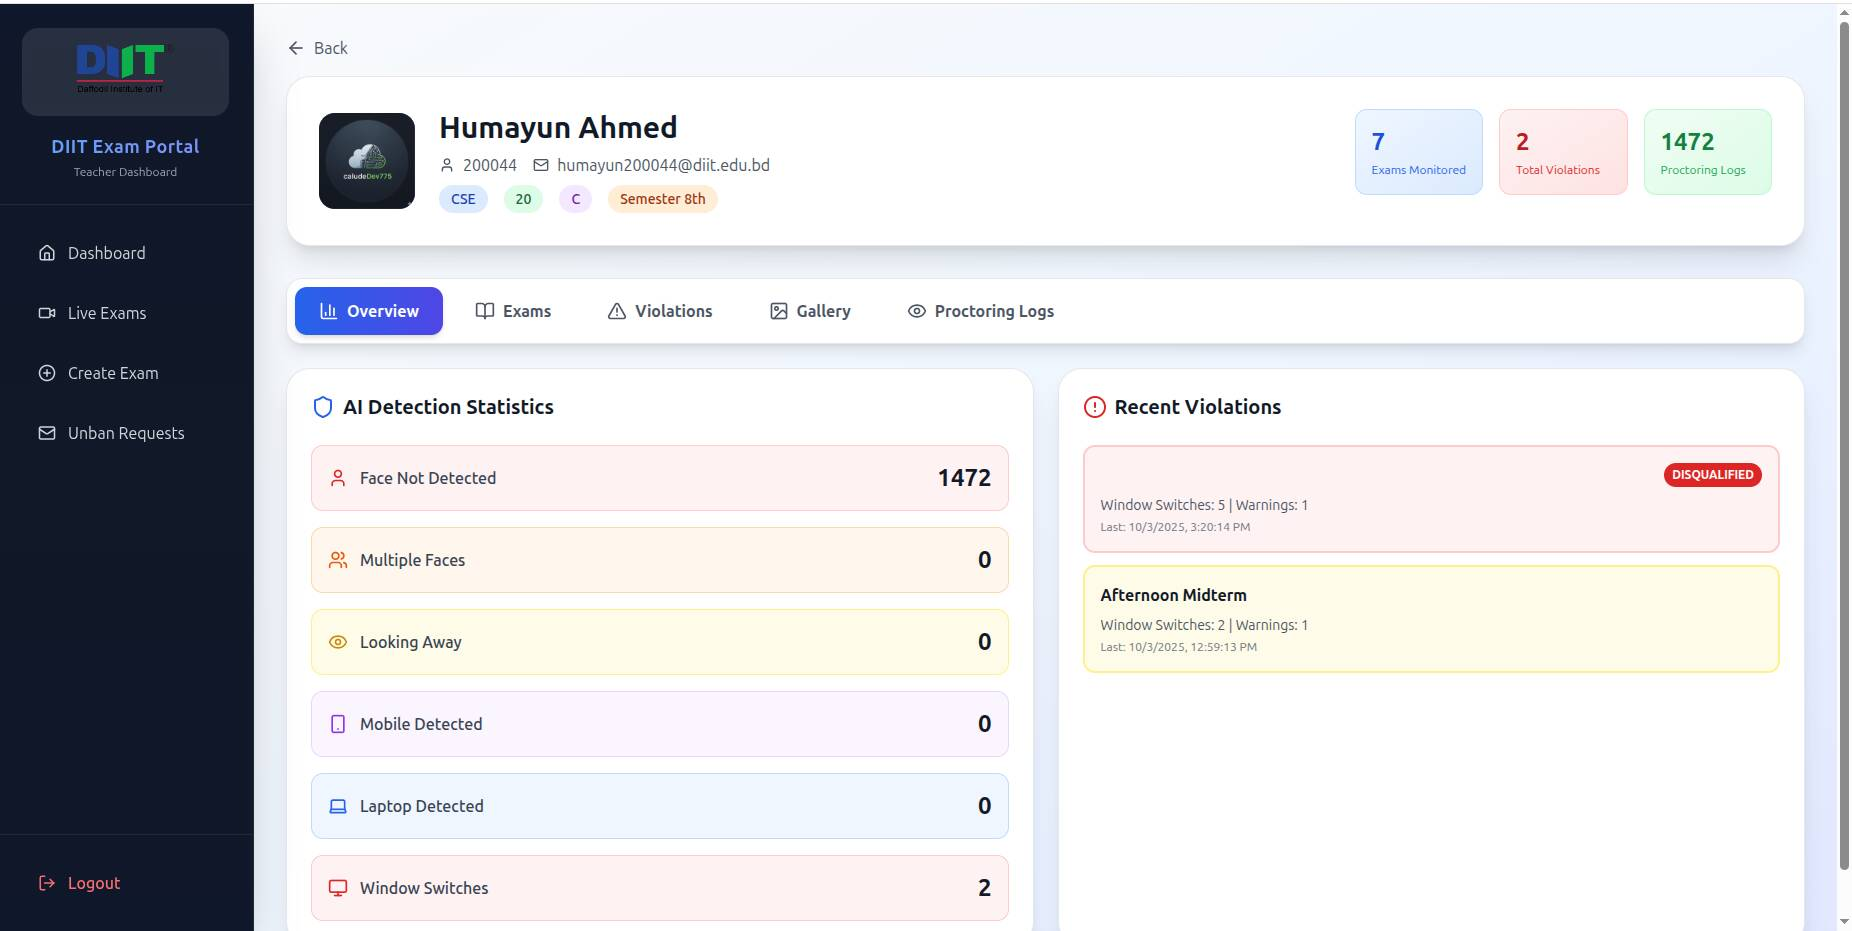
\includegraphics[width=0.7\textwidth]{Chap4/teacher_results_overview.jpg}
    \caption{Results Overview - Exam Performance Metrics}
    \label{fig:teacher_results}
\end{figure}

\begin{figure}[p]
    \centering
    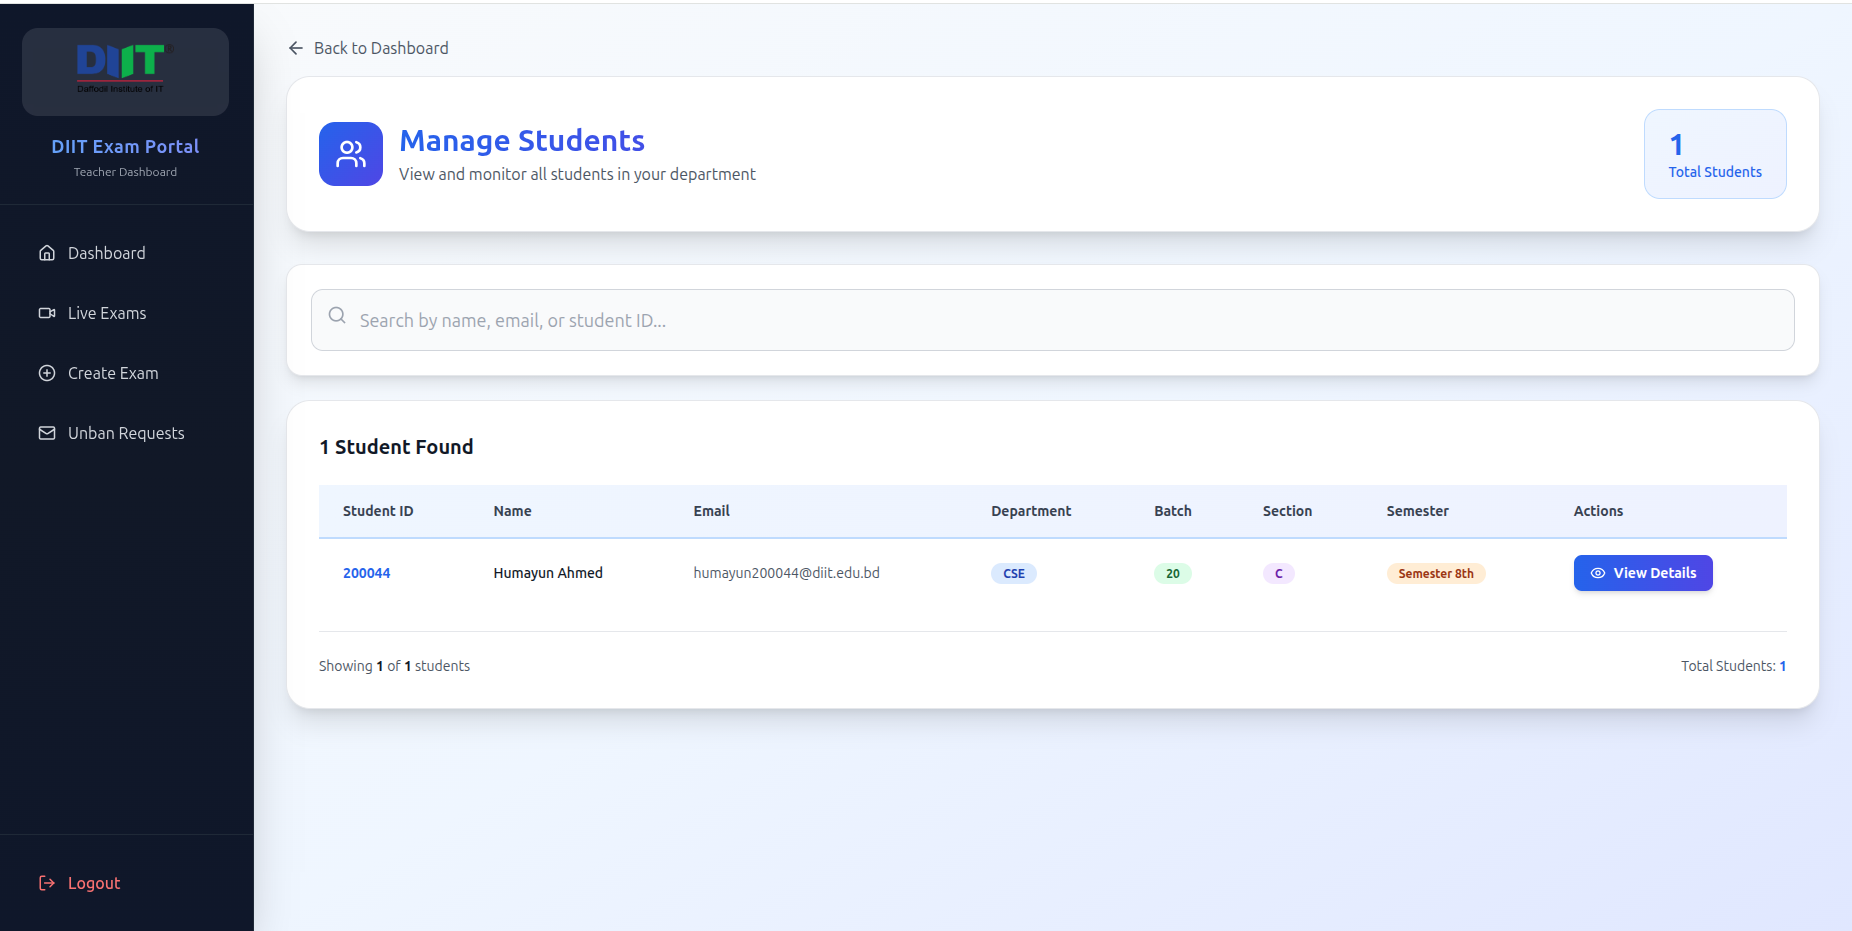
\includegraphics[width=0.7\textwidth]{Chap4/teacher_students.png}
    \caption{Students Management - Class Overview}
    \label{fig:teacher_students}
\end{figure}

\subsection{Unban Requests}

Teachers review student appeals for violations with violation history and snapshots. When students are banned due to excessive violations, they can submit unban requests with explanations. Teachers can review the complete violation history, view captured snapshots during violations, and make decisions to approve or reject the appeal.

\begin{figure}[p]
    \centering
    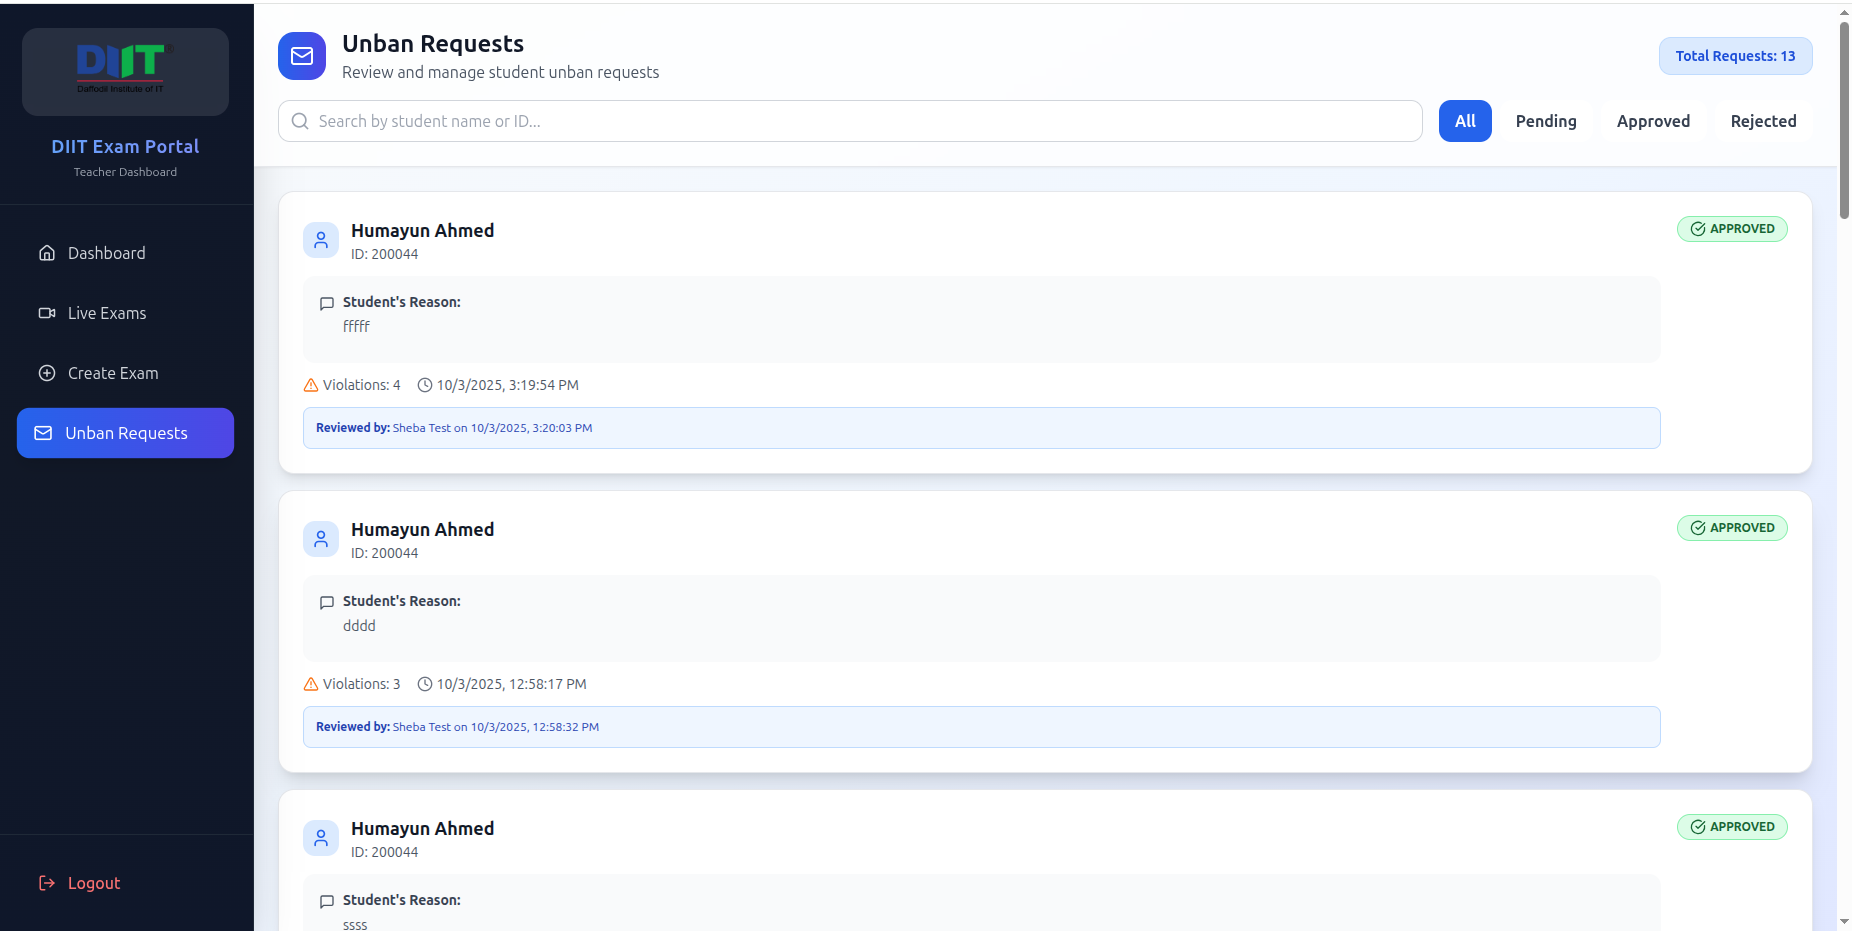
\includegraphics[width=0.7\textwidth]{Chap4/teacher_unban_requests.png}
    \caption{Unban Requests - Student Appeals Review}
    \label{fig:teacher_unban}
\end{figure}

\section{Student Dashboard}

The Student Dashboard provides access to assigned exams, proctored exam-taking with real-time AI monitoring, and performance tracking. Students see upcoming exam cards with countdown timers, recent exam history with scores, performance summary graphs, and notification center for important updates.

\begin{figure}[p]
    \centering
    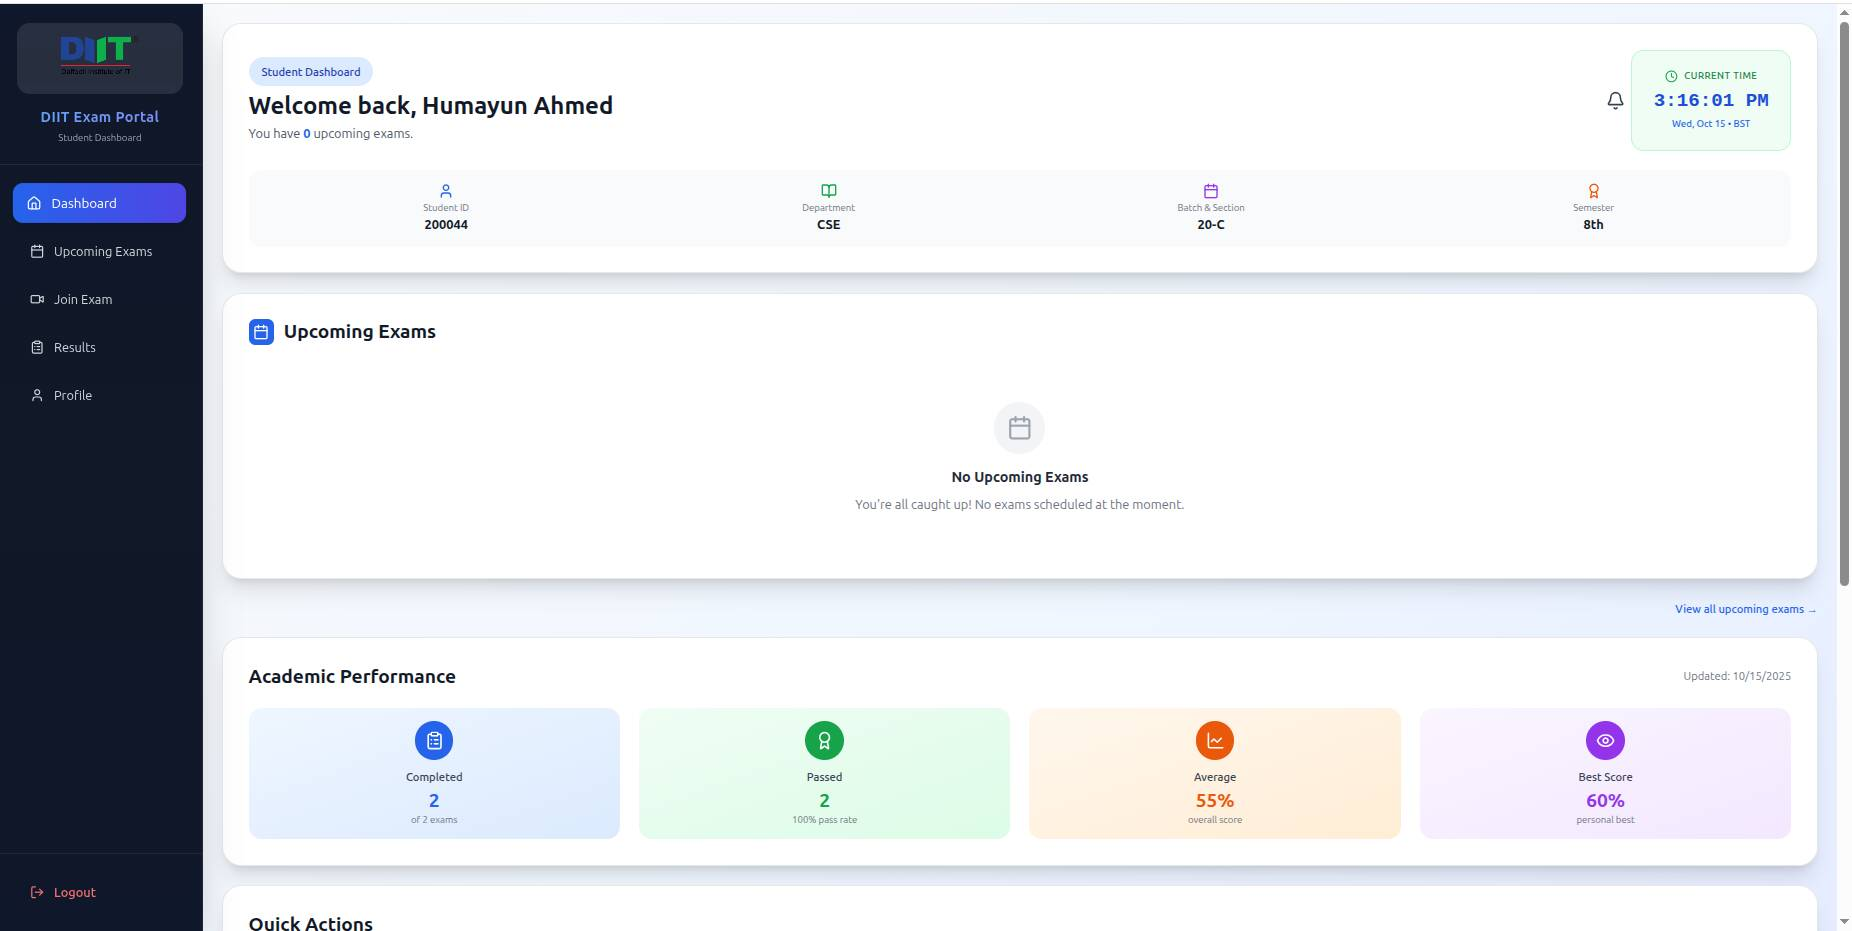
\includegraphics[width=0.8\textwidth]{Chap4/student_dashboard_overview.jpg}
    \caption{Student Dashboard Overview}
    \label{fig:student_dashboard}
\end{figure}

\subsection{Exam Setup and Camera Configuration}

Students complete system compatibility checks and optionally set up mobile camera using QR code pairing. Before starting an exam, students must pass system checks for camera availability, browser compatibility, network connectivity, and system requirements. For enhanced monitoring, students can enable dual camera mode by scanning a QR code with their mobile device to provide an additional viewing angle.

\begin{figure}[p]
    \centering
    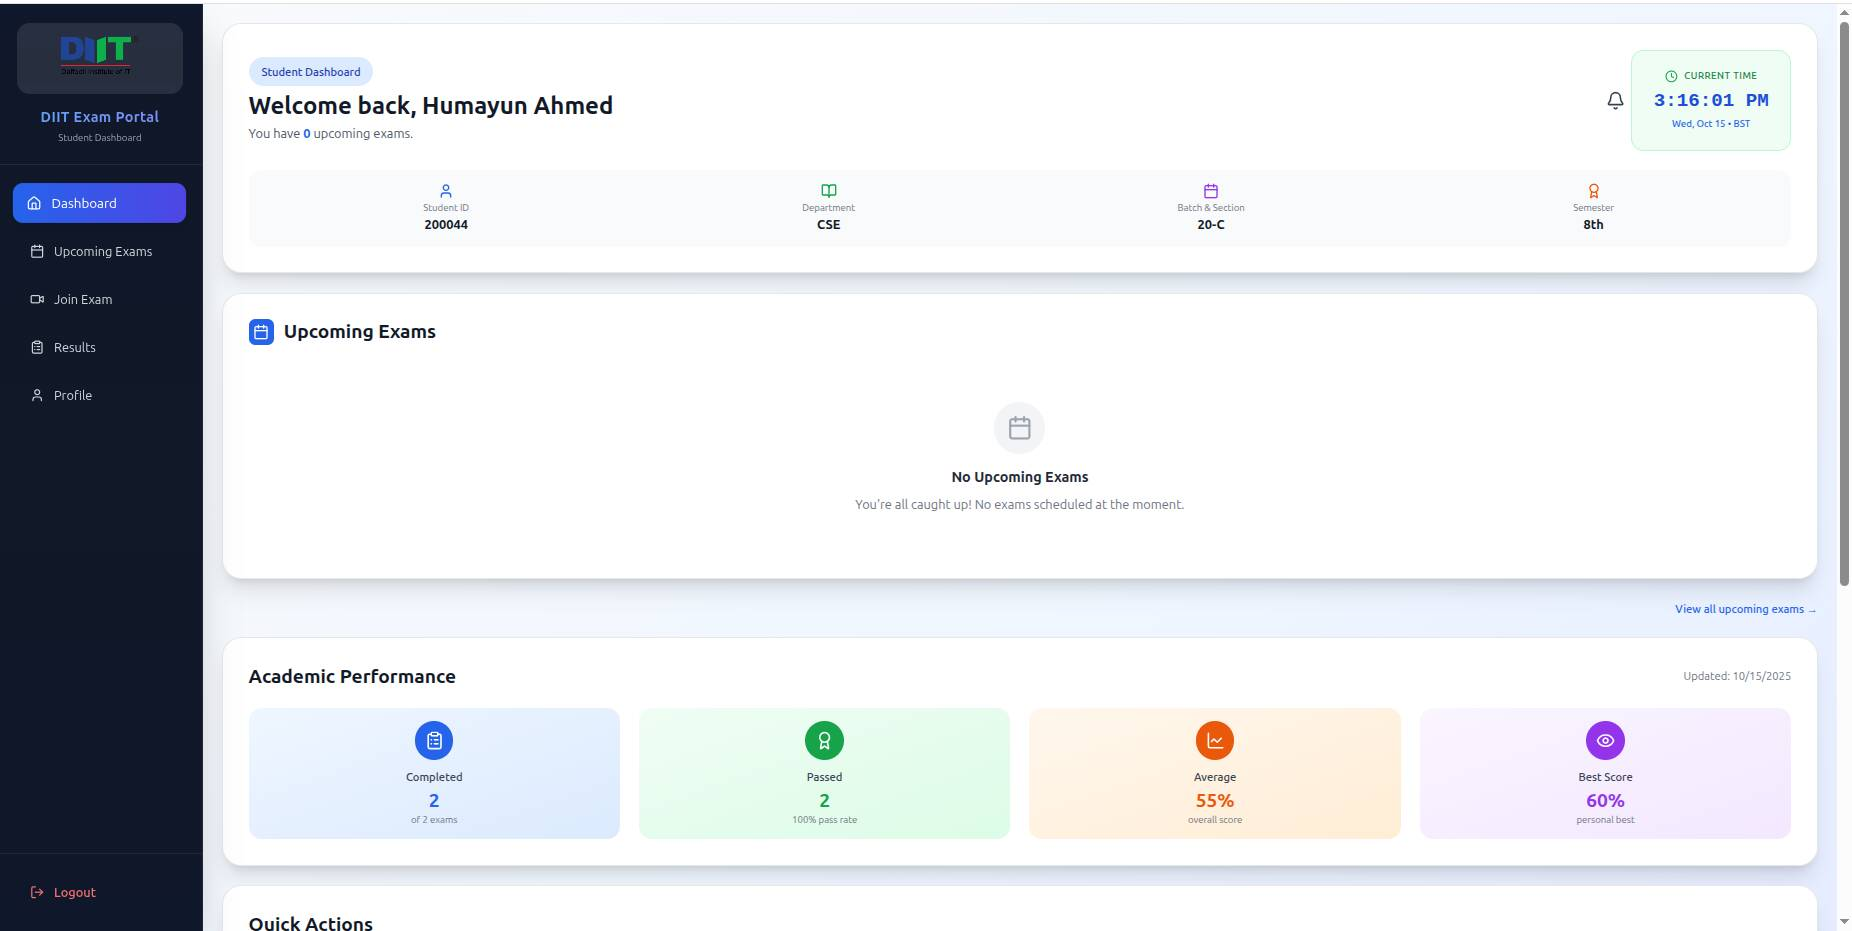
\includegraphics[width=0.8\textwidth]{Chap4/student_mobile_camera_setup.jpg}
    \caption{Mobile Camera Setup - QR Code Pairing for Dual Camera Mode}
    \label{fig:student_camera}
\end{figure}

\subsection{Taking Proctored Exam}

The exam interface includes header with timer, question display panel, and proctoring monitor with live camera feed. Students see their current question with multiple choice options or text input for written answers, a timer counting down remaining time, navigation buttons, and a question palette showing attempted/unattempted status. The proctoring monitor displays the live camera feed with AI analysis status, current accuracy score (0-100\%), real-time violation warnings, and violation counter. Students receive immediate feedback through visual indicators, pop-up warnings for detected violations, and accuracy score updates.

\begin{figure}[p]
    \centering
    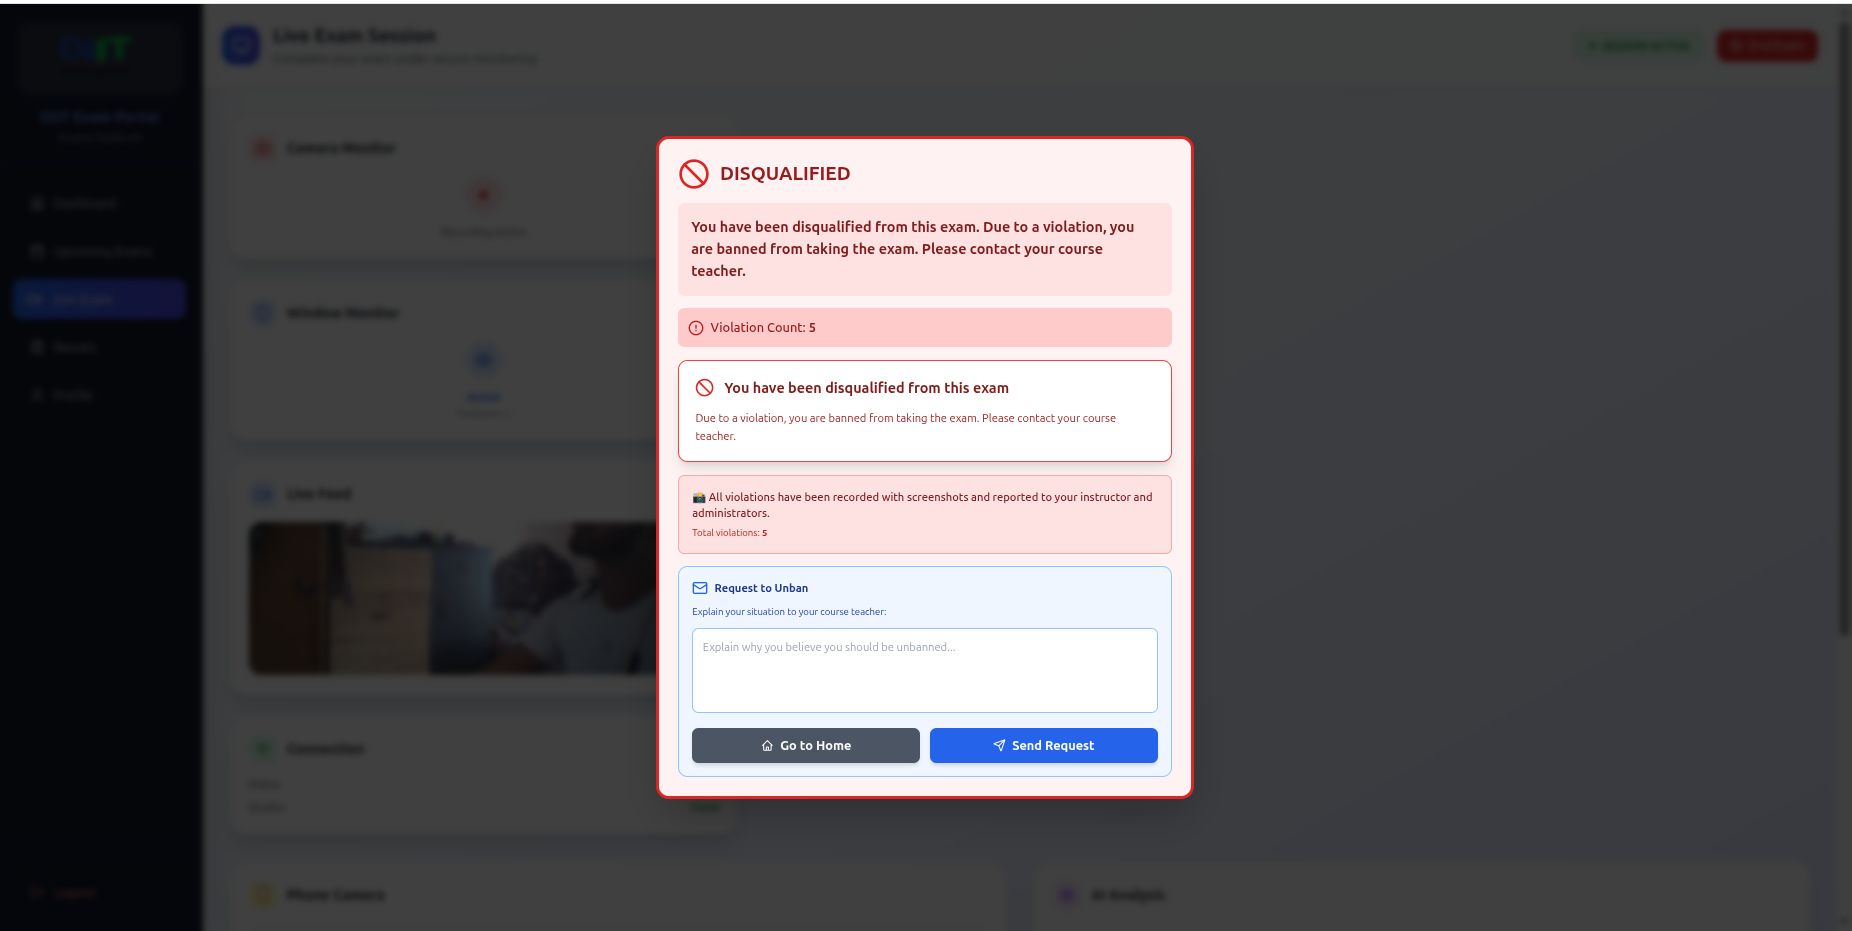
\includegraphics[width=0.7\textwidth]{Chap4/student_exam_interface.png}
    \caption{Exam Interface - Question Display and Timer}
    \label{fig:student_exam}
\end{figure}

\begin{figure}[p]
    \centering
    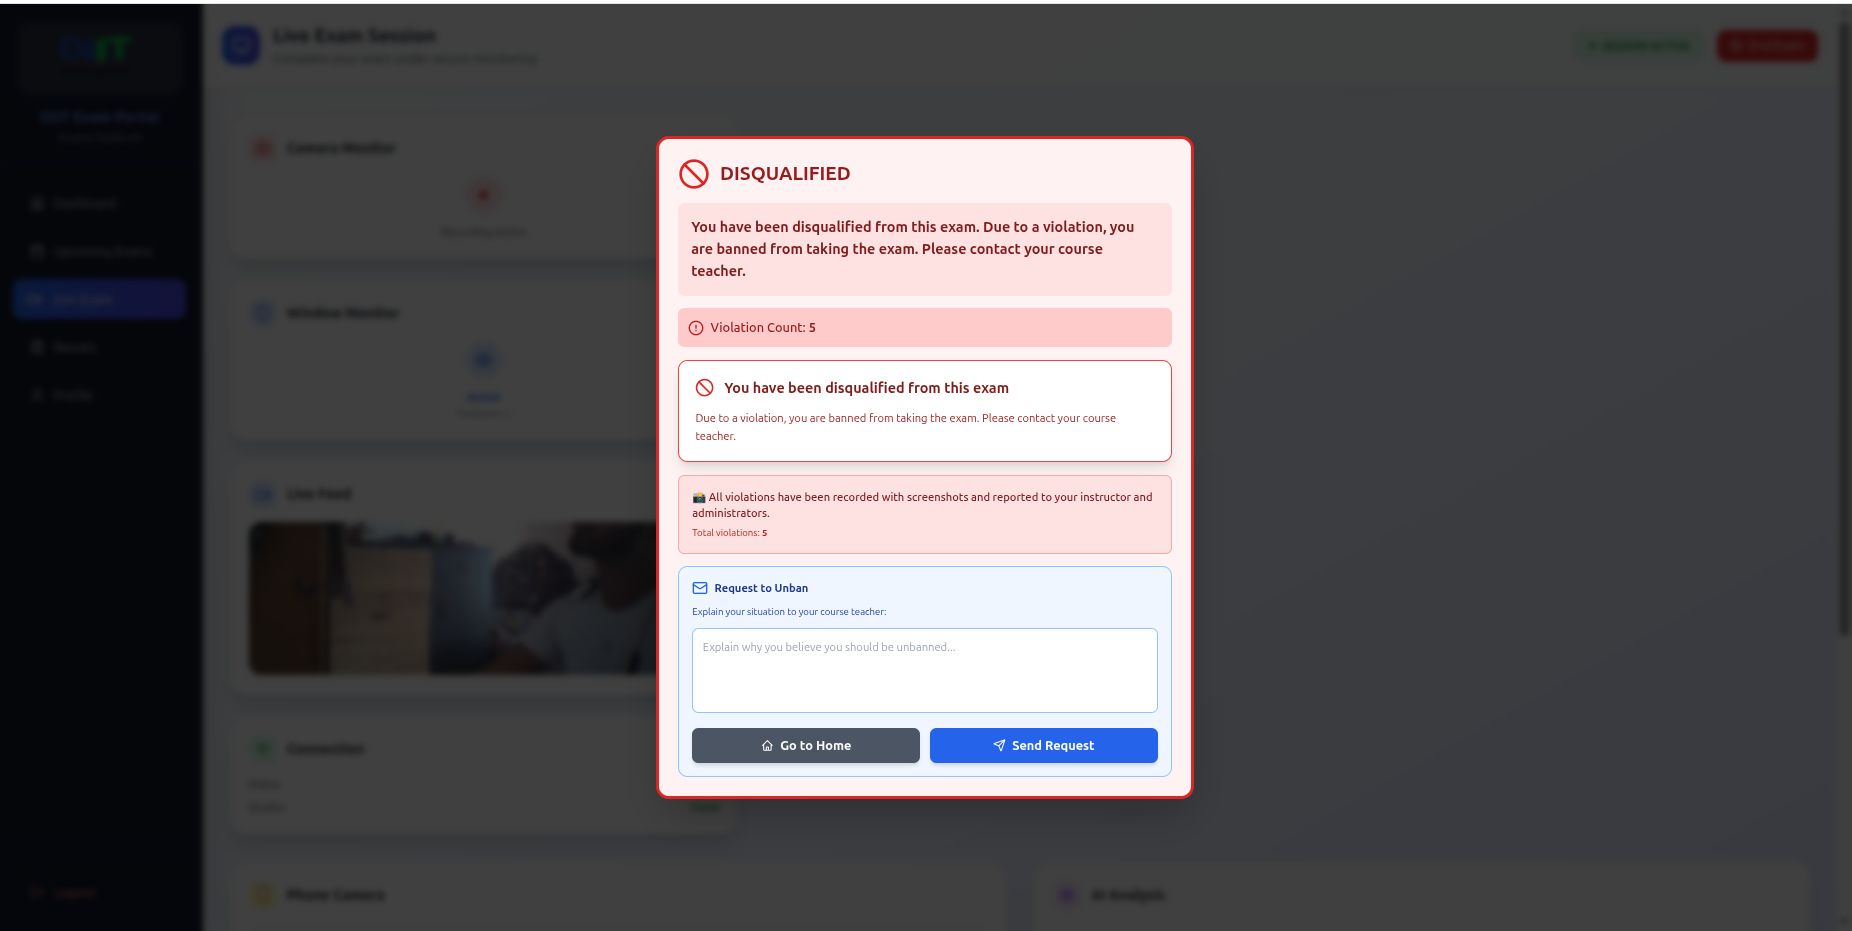
\includegraphics[width=0.7\textwidth]{Chap4/student_proctoring_feedback.png}
    \caption{Proctoring Feedback - Real-time AI Monitoring}
    \label{fig:student_feedback}
\end{figure}

\subsection{Exam History and Profile}

Students view complete exam history with filtering options and manage personal profile. The exam history section displays all past exams with dates, scores, violation counts, and status (passed/failed/pending). Students can filter by date range, course, or exam type. The profile section allows students to update personal information, academic details, change password, and manage notification preferences.

\begin{figure}[p]
    \centering
    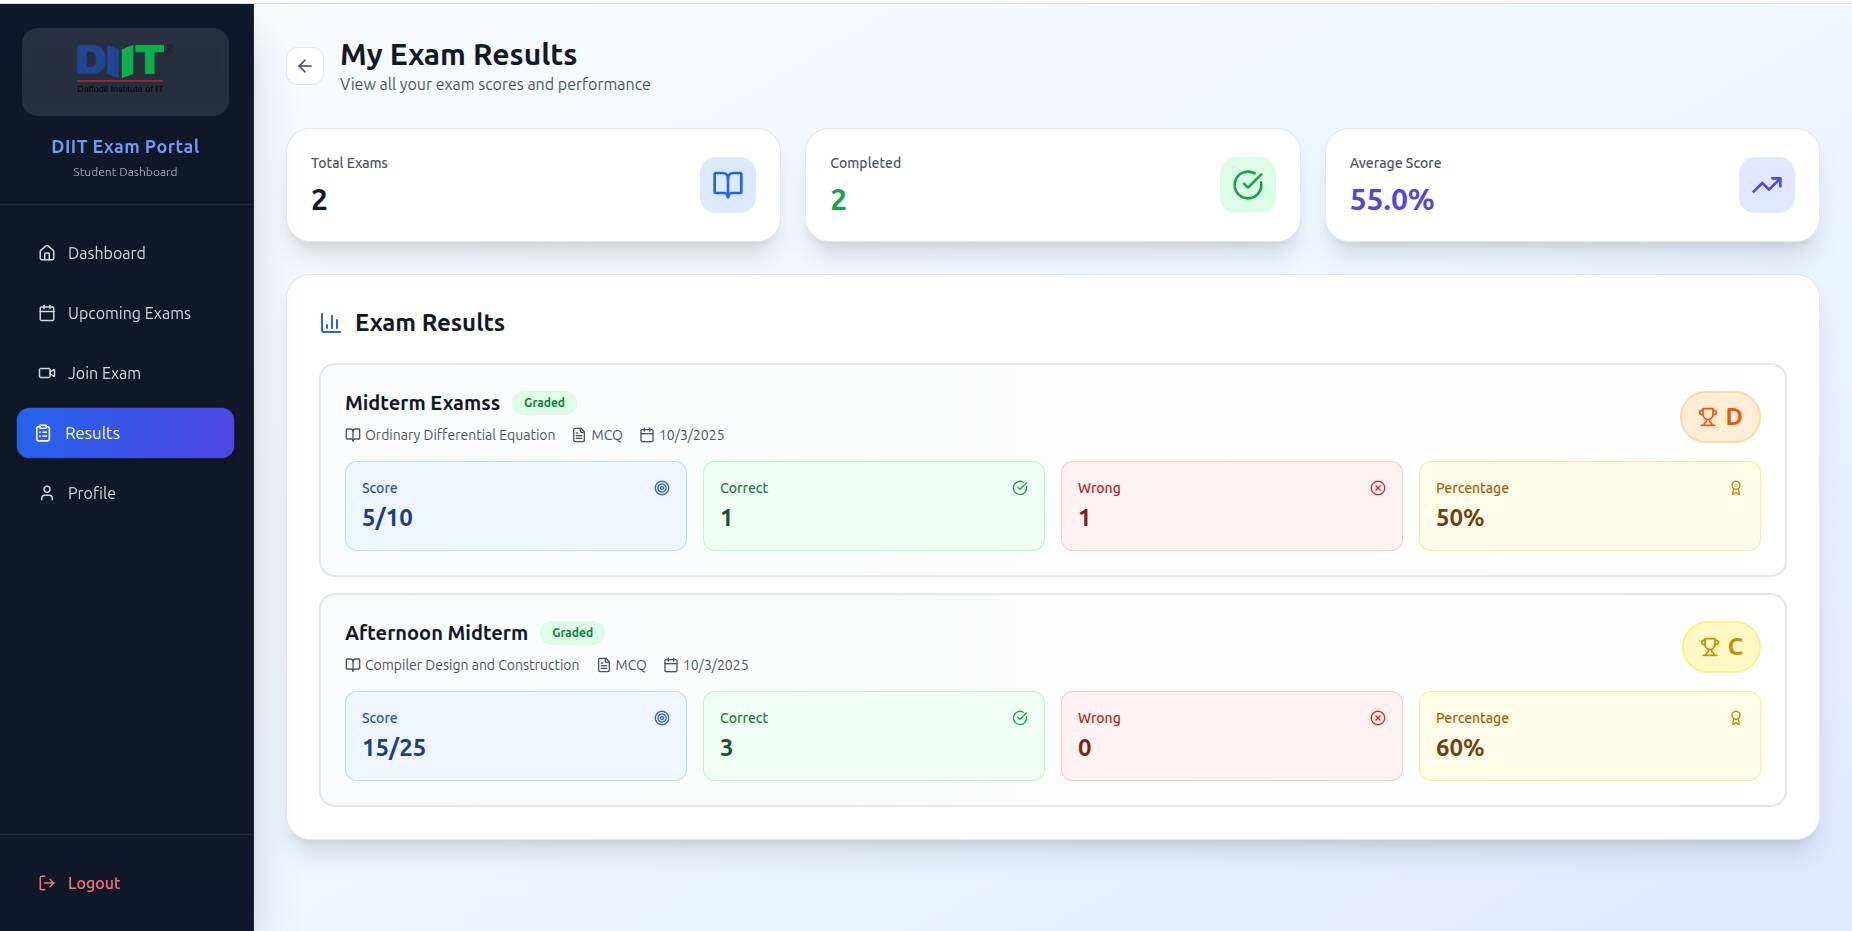
\includegraphics[width=0.7\textwidth]{Chap4/student_exam_history.jpg}
    \caption{Exam History - Past Performance Records}
    \label{fig:student_history}
\end{figure}

\begin{figure}[p]
    \centering
    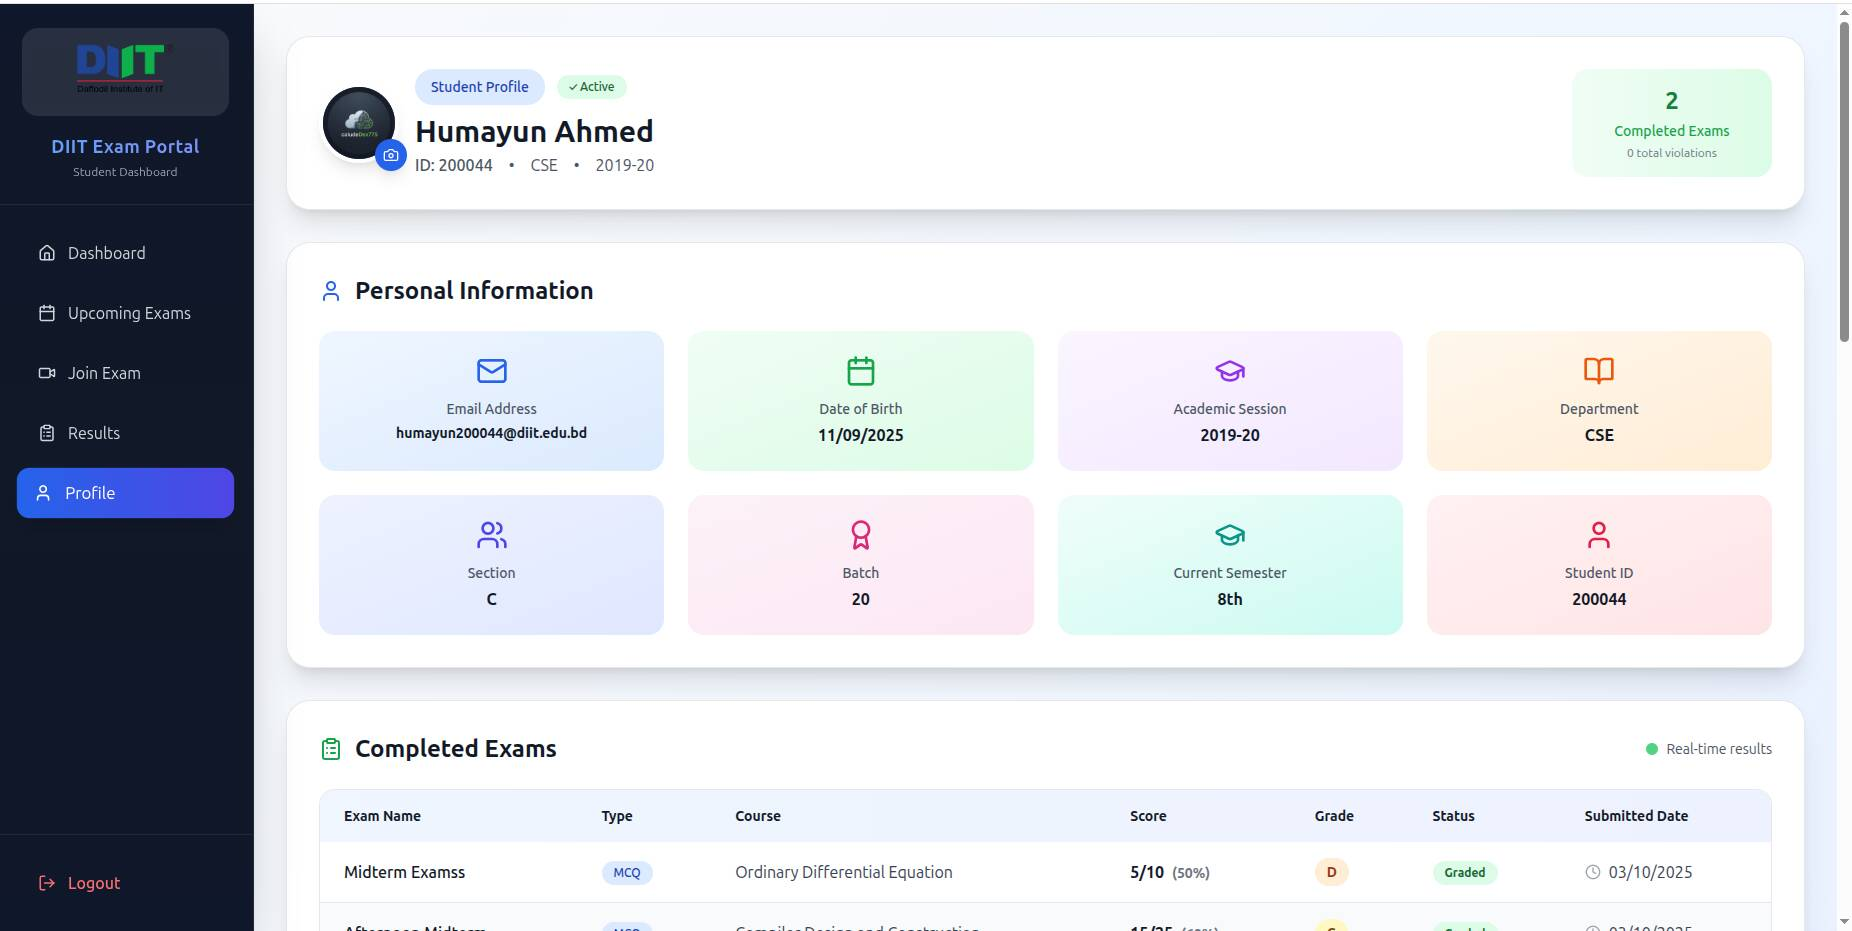
\includegraphics[width=0.7\textwidth]{Chap4/student_profile.jpg}
    \caption{Student Profile - Personal Information Management}
    \label{fig:student_profile}
\end{figure}

\section{Summary}

This chapter presented the complete implementation of the AI-Powered Online Exam Proctoring System with role-based interfaces for Admin, Teacher, and Student users. The system integrates modern web technologies (React 19.0, Flask 3.1.1), AI models (YOLOv8n, MediaPipe), and real-time communication (WebRTC, Socket.IO) to deliver a robust proctoring solution. Key achievements include multi-step exam creation, dual camera support with QR code pairing, real-time violation detection with 8-level priority system, live monitoring dashboard with grid view, automated and manual grading capabilities, and comprehensive user management with appeal processes.
